\documentclass[12pt]{article}

% Language setting
% Replace `english' with e.g. `spanish' to change the document language
\usepackage[english]{babel}

% Set page size and margins
% Replace `letterpaper' with `a4paper' for UK/EU standard size

\usepackage[top=3cm,bottom=3cm,left=3cm,right=3cm,marginparwidth=1.75cm]{geometry}
	
% Load the setspace package
\usepackage{setspace}
\usepackage{amsmath}
\usepackage{listings}
\usepackage{xcolor}

\lstdefinestyle{mystyle}{
    commentstyle=\color{gray},
    keywordstyle=\color{blue},
    numberstyle=\tiny\color{gray},
    stringstyle=\color{purple},
    basicstyle=\ttfamily\footnotesize,
    breakatwhitespace=false,         
    breaklines=true,                 
    captionpos=b,                    
    keepspaces=true,                 
    numbers=left,                    
    numbersep=5pt,                  
    showspaces=false,                
    showstringspaces=false,
    showtabs=false,                  
    tabsize=2
}

\lstset{style=mystyle}

% Useful packages
\usepackage{amsmath}
\usepackage{graphicx}
\usepackage[colorlinks=true, allcolors=blue]{hyperref}
\usepackage{tikz}
\usepackage{natbib}
\doublespacing

\bibliographystyle{unsrtnat}

\usetikzlibrary{shapes.arrows, positioning, arrows.meta}


\title{Theoretical framework}
\author{Riccardo Dal Cero}

\begin{document}

\maketitle

\begin{abstract}
    The main idea is to study how and whether the asymmetry of information have an impact on the cleansing effect of
    recession, replicating the model in computer  simulation.
\end{abstract}
\section{Introduction} 
In macroeconomic theory, the investigation of business cycles and long-term growth trajectories traditionally unfolds in
distinct academic silos, drawing a parallel to the distinct realms of quantum mechanics and Einstein's theory of
relativity in physics. This academic segregation, however, obscures a fundamental and profound question: How do business
cycles influence long-term economic growth? The exploration of this question is more than an academic exercise; it
underpins the practical understanding of short-term economic policies, such as automatic stabilizers, and their profound
long-term impacts on the economy. 

Embarking on this exploration, my research primarily dwells in the realm of theory, supplemented by rigorous simulation
and calibration exercises. The intricate complexity of business cycles, particularly evident during periods of economic
downturn and recovery, challenges empirical approaches due to the plethora of confounding variables. Thus, a theoretical
lens, rather than a purely empirical one, is employed to dissect and understand these phenomena. 

Central to this theoretical framework is an examination of the role of financial market frictions during economic
recessions. A key inquiry here is the investigation of policy interventions, such as demand stabilizers, and their
potential effect in attenuating the 'cleansing effect' of recessions. This exploration is pivotal in understanding
whether such policies might inadvertently lead to a reduced economic baseline or steady state in the long term. 
 
The conceptual foundation of this investigation is inspired by an ecological analogy  the cyclical dynamics observed
between predator and prey populations in nature. This natural cycle, when observed over extended periods, reveals not
just self-contained oscillations but also underlying trends of population growth for both predators and prey. This
observation leads to a compelling analogy for economic cycles: while they appear as short-term fluctuations, they might
be underpinned by long-term growth trajectories. 

In natural ecosystems, interventions aimed at stabilizing these cycles  such as protecting prey during times of
increased predation  might seem beneficial in the short term. However, such interventions often neglect the critical and
natural process of selection. This interference disrupts evolutionary mechanisms, potentially leading to unforeseen
consequences over time, such as the propagation of traits detrimental to the species' survival and adaptability in
changing environments. 

My thesis extends this analogy to the economic sphere, positing a similar selective mechanism at play in economic
systems. The primary focus is on the recession's cleansing effect, which might be analogous to natural selection in
ecology. This effect could potentially 'weed out' less productive firms, leaving a market landscape dominated by more
efficient players. The exploration aims to decipher whether such an economic 'natural selection' mechanism exists and,
if so, how it shapes the fabric of productivity, innovation, and growth in the long term. Through this lens, the
research endeavors to contribute a nuanced understanding of the intricate interplay between short-term economic
fluctuations and long-term economic evolution, offering insights into the design and implications of economic policies. 
In the following sections, we will delve deeper into specific theories that bridge the gap between business cycles and
long-term economic growth. However, it is beneficial first to embark on a brief historical journey through the evolution
of thought regarding business cycles, to understand the context and development of these interconnected economic
theories. This exploration will provide a foundation for appreciating the diversity of perspectives and the progression
of ideas that have shaped our understanding of the intricate relationship between short-term economic fluctuations and
long-term growth trajectories. 

\section{Business cycle history}

The exploration of business cycle theories represents a cornerstone in the history of economic thought. A prominent
exponent in this realm was Friedrich Hayek, who articulated the complexities of business cycles in relation to economic
equilibrium theory. Hayek's perspective is encapsulated in his own words: 

\begin{quote}
    "The incorporation of cyclical phenomena into the system of economic equilibrium theory, with which they are in
    apparent contradiction, remains the crucial problem of Trade Cycle theory; 
    By 'equilibrium theory' we primarily understand the modern theory of the general interdependence of all economic
    quantities, which has been perfectly expressed by the Lausanne School of theoretical economics." \cite{Hay33} 
\end{quote}


In the turbulent era of the early 1930s, the exploration of business cycles was prominently shaped by the contrasting
viewpoints of Friedrich Hayek and John Maynard Keynes, two of the twentieth century's most influential economists.
Hayek's examination of business cycles, as delineated in his seminal work "Monetary Theory and the Trade Cycle,"
\cite{Hay33}, and further elaborated in "The Pure Theory of Capital" \cite{Ha41}, provides a profound analysis
through the lens of monetary theory and its ramifications on capital structure. Hayek posited that economic distortions,
notably those stemming from the artificial depression of interest rates by central banks, precipitate malinvestments
during periods of economic expansion. These malinvestments, especially prevalent in capital-intensive sectors, were
deemed unsustainable, leading inevitably to economic downturns characterized by the correction of these misallocations. 

Conversely, Keynes, in his groundbreaking "The General Theory of Employment, Interest, and Money" \cite{Key36},
approached the business cycle issue from an equilibrium perspective, focusing on the role of aggregate demand in
determining overall economic activity levels. Keynes argued that a shortfall in aggregate demand could lead to
protracted periods of high unemployment, advocating for active government intervention to stimulate demand and
re-establish economic equilibrium. 

Hayek's theoretical framework underscores the intricate relationship between capital investment and monetary
disequilibrium within the business cycle. He elucidates this connection through the concept of inter-temporal
preferences, which dictate the pace of capital investment and the extent of capital accumulation. The decision-making
process regarding the allocation of resources between present consumption and future investment is critical to
understanding the cyclical nature of the economy. Hayek asserts: 

\[ I_t = f(r_t, r_n) \]
\[ r_t < r_n \rightarrow \text{Malinvestment} \]

where \( I_t \) signifies investment at time \( t \), \( r_t \) represents the market interest rate, and \( r_n \)
denotes the natural rate of interest. A divergence between \( r_t \) and \( r_n \), particularly when \( r_t \) is
artificially maintained below \( r_n \), leads to malinvestments. This discrepancy between the market and natural rates
of interest, exacerbated by the expansion of bank credit, serves as the cornerstone of Hayek's business cycle theory.
Hayek further elaborates on the dynamic and temporal aspects of production and investment in "The Pure Theory of
Capital" \cite{Ha41}, where he critically assesses the equilibrium-based economic theories and emphasizes the
importance of understanding the temporal structure of capital. 

Hayek's analysis of monetary disequilibrium and its impact on the business cycle is complemented by his insights into
the mechanisms of bank credit creation and its influence on the natural state of equilibrium in the market for loanable
funds. The expansion of bank credit, which decouples the market rate of interest from the natural rate, instigates
cycles of over-investment and mal-investment, ultimately culminating in inter-temporal economic instability. 

These theoretical perspectives offered by Hayek provide a nuanced understanding of the complexities inherent in the
business cycle, challenging the Keynesian emphasis on aggregate demand and fiscal policy interventions. Hayek's
contributions, particularly in "The Pure Theory of Capital," highlight the significance of capital theory in analyzing
monetary disequilibria and underscore the dynamic and inter-temporal nature of economic activities. 

Thus, while Keynes emphasized stabilizing aggregate demand to achieve equilibrium and mitigate business cycles, Hayek
focused on the inherent dynamism and complexity of economic systems, criticizing equilibrium models for their
oversimplification of the intricate processes that drive economic activities. This divergence in views marked a
fundamental debate in economic theory, shaping the discourse on how economies respond to and recover from periods of
economic downturns. 
\par
\vspace{2cm}
Joseph Schumpeter, another influential economist of the early 20th century, brought a unique perspective to the
discussion of business cycles, one that diverged significantly from both Hayek and Keynes. Schumpeter's approach,
primarily outlined in his theory of "creative destruction," emphasized the role of innovation and entrepreneurial spirit
in economic development and business cycles.  

Schumpeter viewed business cycles as inherent and vital to capitalist economies, driven by the process of innovation.
According to Schumpeter, the entrepreneur is the agent of change, introducing new technologies, products, and methods,
which disrupt existing market equilibria. This process of innovation leads to the destruction of outdated industries and
economic structures, paving the way for new ones. In Schumpeter's framework, the cyclical nature of the economy was a
reflection of this ongoing process of creative destruction, where periods of economic downturns were seen not just as
phases of correction, as Hayek might argue, or as failures of demand, as per Keynes, but as essential for clearing away
the old to make way for the new. 

While Hayek focused on the distortions in capital structure caused by monetary interventions and Keynes emphasized the
role of aggregate demand and government intervention in stabilizing the economy, Schumpeter's perspective highlighted
the evolutionary nature of capitalist economies. He argued that economic fluctuations were natural and necessary, a
process through which economies evolve and adapt over time. Schumpeter's theory thus provided a more dynamic view of
capitalism, recognizing the disruptive yet progressive role of innovation and entrepreneurship in shaping economic
landscapes. 

Schumpeter's contribution added a dimension of evolutionary change to the understanding of business cycles,
contrasting with Hayek's emphasis on monetary theory and capital structure, and Keynes's focus on equilibrium and
aggregate demand. Schumpeter's insights into the transformative power of innovation offered a more optimistic view of
economic downturns, seeing them as opportunities for new growth and advancements. 
 
In the aftermath of World War II, the landscape of macroeconomic theory experienced a paradigmatic shift, significantly
influenced by the ascendancy of Keynesian economics. The widespread devastation of the war necessitated a thorough
reevaluation of economic policies and theories, setting the stage for Keynesian principles to take a dominant position
in shaping government approaches to economic policy, especially concerning business cycles. 

Central to the Keynesian doctrine is the advocacy for proactive government intervention to stabilize economic cycles.
This perspective gained substantial traction in the post-war era, a period marked by the reconstruction efforts of
numerous nations. The foundational principle of Keynesianism, as articulated in Keynes's seminal work "The General
Theory of Employment, Interest, and Money," \cite{key60}is that government spending can act as a catalyst to stimulate demand during
economic downturns. This tenet represented a stark divergence from the pre-war classical economic thought, which
predominantly favored limited government intervention in the economy. 

A key element in Keynesian policy is the concept of fiscal multipliers, which posits that government spending has a
multiplied effect on overall economic output. The multiplier effect can be conceptualized as follows: 

\[ \Delta Y = \text{Multiplier} \times \Delta G \]

where \( \Delta Y \) represents the change in total output, and \( \Delta G \) is the change in government spending. The
'Multiplier' is defined as: 

\[ \text{Multiplier} = \frac{1}{1 - c(1 - t) + m} \]

Here, \( c \) is the marginal propensity to consume, \( t \) is the tax rate, and \( m \) is the marginal propensity to
import. This formula illustrates how an increase in government spending (\( \Delta G \)) can lead to a larger increase
in total output (\( \Delta Y \)), thereby stimulating economic activity during recessions. 

The immediate post-war period witnessed the successful implementation of Keynesian policies, evidenced by stable
economic growth and reduced unemployment rates. This success solidified the influence of Keynesian economics,
particularly in the United States and Western Europe, where governments widely adopted strategies such as fiscal
stimulus, interest rate manipulation, and welfare state expansion to regulate economic cycles and mitigate recessionary
impacts. 

The era also saw the rise of the concept of "fine-tuning" the economy. Policymakers and economists believed that through
judicious management of fiscal and monetary policies, it was possible to circumvent severe economic downturns and
maintain consistent growth. The underlying idea was that by modulating government spending, tax policies, and interest
rates, governments could bolster and sustain demand, thereby smoothing out the fluctuations inherent in business cycles. 

The post-war dominance of Keynesian economics encountered a significant challenge in the 1970s with the onset of
stagflation, a term coined to describe the unprecedented combination of high inflation and high unemployment,
accompanied by stagnant demand. This phenomenon posed a critical challenge to the Keynesian framework, which had not
anticipated such a simultaneous occurrence of inflation and stagnation, fundamentally questioning its policy
prescriptions. 

The Keynesian model, as traditionally understood, posited an inverse relationship between inflation and unemployment,
often illustrated by the Phillips Curve \cite{Phi58}. This relationship suggested that higher inflation could help reduce
unemployment by stimulating demand, and vice versa. However, the stagflation of the 1970s, where high inflation
coexisted with high unemployment, contradicted this established Keynesian principle. The phenomenon was first brought to
widespread attention by economists such as Milton Friedman and Edmund Phelps, who argued that the Phillips Curve could
only function in the short term, and that long-term attempts to exploit this trade-off would lead to ever-increasing
rates of inflation without reducing unemployment \cite{Fri72}. 

The stagflation era was marked by several critical global events that influenced economic conditions. The 1973 oil
crisis, triggered by an oil embargo by OPEC nations, led to a dramatic increase in oil prices, contributing
significantly to inflationary pressures worldwide. This external shock, coupled with the already expansionary fiscal and
monetary policies in many Western economies, exacerbated inflation without spurring economic growth or reducing
unemployment. 

The Keynesian approach, which advocated for increased government spending and lower interest rates to combat recessions,
appeared ineffective in addressing the simultaneous challenges of stagnation and inflation. This inadequacy led to the
rise of alternative economic theories, such as monetarism and supply-side economics, which focused more on controlling
inflation and stimulating supply rather than managing demand. Monetarism, championed by Milton Friedman, emphasized the
importance of controlling the money supply to manage inflation, arguing that inflation was primarily a monetary
phenomenon\cite{Fri72}. Meanwhile, supply-side economics advocated for reducing tax rates and decreasing regulation to encourage
production and investment. 

The emergence of stagflation and the subsequent paradigm shift in economic theory underscored the complexity of economic
systems and the limitations of existing models. It marked a transition in macroeconomic thought and policy, from a
predominantly Keynesian consensus to a more diverse array of approaches, including monetarism and supply-side economics,
each offering different perspectives on how to achieve economic stability and growth. This period of economic rethinking
paved the way for significant policy shifts in the 1980s, particularly in the United States and the United Kingdom,
where there was a move towards deregulation, reduction of government intervention, and a greater emphasis on monetary
policy to control inflation. 

The narrative of economic thought in the latter half of the 20th century took a pivotal turn with the introduction of
the Lucas Critique, formulated by economist Robert Lucas in 1976 \cite{Luc76}. This critique fundamentally challenged the prevailing
Keynesian orthodoxy and ushered in a new era in the understanding of economic policy and business cycles. 

The Lucas Critique posited that traditional Keynesian macroeconomic models, which were used to design economic policies,
were fundamentally flawed because they did not take into account the way people's expectations and decisions would
change in response to policy shifts. Lucas argued that individuals and firms adjust their behavior based on their
expectations of future policy, which in turn alters the effectiveness of that policy. This meant that historical data,
which Keynesian models heavily relied upon, could not reliably predict the outcomes of economic policies, as the  very
implementation of these policies would change the economic environment and behavior of agents within it.

Consider a simple Keynesian macroeconomic model where output is determined by:
\begin{equation}
    Y_t = \alpha + \beta G_t + \epsilon_t
\end{equation}
where \(Y_t\) is the output, \(G_t\) is the government expenditure, \(\alpha\) and \(\beta\) are parameters, and
\(\epsilon_t\) is a random error term. 

Lucas argued that the parameters \(\alpha\) and \(\beta\) in such models are not constant but change with policy. Thus,
a policy change that alters \(G_t\) will also change \(\alpha\) and \(\beta\), rendering predictions based on historical
data unreliable. This is because the parameters are not deep structural parameters but are themselves functions of
agents' expectations and behaviors, which are influenced by policy. 

The critique can be formalized as follows:
\begin{equation}
    Y_t = f(G_t, \theta_t) + \epsilon_t
\end{equation}
where \(\theta_t\) represents the agents' expectations and behaviors, which are influenced by policies. Therefore, any
policy change that alters \(G_t\) also changes \(\theta_t\), and thus the relationship between \(Y_t\) and \(G_t\). 

The Lucas Critique led to the development of models with microeconomic foundations and rational expectations, where
policy effectiveness is assessed by considering how policies alter agents' expectations and decision-making processes.
This shift was instrumental in the evolution of New Keynesian economics, which integrates rational expectations with
menu costs, nominal rigidities, and other market imperfections. 

The implications of the Lucas Critique were profound. It suggested that policies based on historical models might be
ineffective or even counterproductive. This critique was a significant factor in shifting the focus of macroeconomic
research from Keynesian models, which emphasized aggregate demand and fiscal policy, to new classical models, which
focused more on microeconomic foundations and the role of rational expectations. 

Lucas's ideas were met with resistance and debate. Opponents, particularly those in the Keynesian camp, argued that
while the critique had merit, it did not invalidate the use of all macroeconomic modeling. They contended that while
expectations are important, other factors like market imperfections and rigidities also play a critical role in the
functioning of the economy. These Keynesian economists argued for the continued relevance of fiscal policy and
government intervention, especially in situations like recessions, where private demand is insufficient. 

The debate sparked by the Lucas Critique led to significant advancements in economic theory. It pushed economists to
develop new models that incorporated rational expectations and more robust microeconomic foundations. This period saw
the rise of New Keynesian economics, which attempted to merge Keynesian concepts with microeconomic foundations,
including rational expectations and market imperfections. 

In the years following the Lucas Critique, economic thought around business cycle theories underwent significant
evolution, particularly with the integration of various types of frictions into macroeconomic models. This period saw a
shift from idealized notions of perfect competition and complete information to models that better reflected the
complexities of real-world economies. 

The late 1980s and early 1990s marked the rise of New Keynesian economics, which emphasized the role of nominal
rigidities, such as sticky prices and wages, in the economy. Pioneering works in this field, like those of Gregory
Mankiw and David Romer \cite{ManRom91}, established theoretical foundations where these market imperfections were central to explaining
why economies do not self-correct efficiently after disturbances.  

Simultaneously, Real Business Cycle (RBC) theory, emerging from the seminal work of Finn E. Kydland and Edward C.
Prescott, particularly their influential paper "Time to Build and Aggregate Fluctuations" \cite{Pre82}, focused on real
(non-monetary) shocks and frictions. RBC theory emphasized aspects such as technology shocks and constraints in capital
accumulation, offering insights grounded in neoclassical microfoundations. 

Another significant development was the exploration of credit market frictions, especially after the financial crisis of
2007-2008. The work of Bernanke and Gertler, particularly "Agency Costs, Net Worth, and Business Fluctuations" \cite{BerGer86},
brought to light how asymmetric information in credit markets could amplify business cycles, linking the financial
health of firms to their investment and production decisions. 

Further, the introduction of search and matching frictions in labor markets, attributed to the work of economists like
Diamond, Mortensen, and Pissarides, highlighted how inefficiencies in matching workers with jobs could lead to
persistent unemployment, thus influencing the business cycle. Their research, including papers like "Job Creation and
Job Destruction in the Theory of Unemployment" (1994)\cite{MorDalPisChr94}, was pivotal in integrating labor market dynamics into business
cycle theories. 

The culmination of these developments is seen in the formulation of Dynamic Stochastic General Equilibrium (DSGE) models
that incorporate various frictions. These models, blending insights from New Keynesian and RBC theories, integrate
sticky prices, financial frictions, and labor market imperfections. They have become a standard tool for economic policy
analysis, particularly among central banks, representing a significant advance in the ability to simulate and understand
economic fluctuations and policy impacts. 

\section{Theories Connecting Business Cycles to Long-Term Growth}

In the domain of economic theory, the relationship between business cycles (BC) and long-term growth is dissected into
two principal schools of thought. The conventional viewpoint suggests that long-term growth is chiefly propelled by
technological progress. Within this framework, technological advancements are often viewed as exogenous—arising outside
the economic model's explanatory scope, as highlighted in the seminal contributions of \cite{Sol56} and \cite{Swa56}.
This perspective treats technological progress as an independent variable that exerts influence on economic growth
without being influenced by the economy's internal dynamics. 

Contrastingly, an alternative strand of theoretical work aims to endogenize technological progress, weaving it into the
fabric of the economic process. These models embed factors such as incentives for innovation, the value of education,
and the accumulation of knowledge through economic activities, epitomizing the 'learning by doing' paradigm. A prominent
example of this approach is found in \cite{Sta90}, which posits technological progress as an emergent property of
economic behavior and incentives, rather than a mysterious external force. 

A critical aspect of the 'learning by doing' model is its premise that technological frontiers are contingent upon the
existing knowledge base, which expands primarily through practical experience. Consequently, periods of economic
expansion witness a sharp increase in the knowledge stock, driven by higher employment levels, whereas recessions tend
to stabilize or even diminish this stock due to reduced employment rates. This dynamic suggests that economies devoid of
cyclical fluctuations might attain a superior steady-state growth, as employment remains consistently high, fostering
continuous technological advancement. From this perspective, the concept of a 'cleansing effect'—whereby economic
downturns eliminate low-productivity jobs and ostensibly strengthen the economy—is challenged. The elimination of even
low-productivity roles can erode the overall knowledge base. 

Such theories reframe the discourse on stabilization policies, particularly fiscal interventions, by highlighting their
role in sustaining employment and, by extension, supporting the technological frontier even in downturns. 

To illustrate this theory's implications more vividly, consider a nuanced example: an antiquated factory with limited
land resources discovers an innovative method to utilize an old tractor more efficiently. Despite the ingenuity of this
breakthrough, if the broader economy has moved beyond the technology that the tractor represents, the innovation might
not significantly contribute to the overall knowledge stock or push the technological frontier forward. This scenario
prompts a fundamental inquiry: does innovation at the lower end of the skill spectrum or within outdated technological
contexts meaningfully advance the technological frontier? Or, would it be more beneficial for economic growth to
transition such small-scale innovations into larger entities equipped with modern technologies? 

One significant critique concerns the disparity in learning opportunities across different sectors and among
individuals. The model's premise of uniform learning opportunities does not always align with the reality that some
industries, such as the technology sector, offer rapid innovation and learning environments compared to more traditional
manufacturing industries, where the pace of learning and innovation may be inherently slower due to the nature of the
work processes involved.

Furthermore, the model may not adequately address the issue of structural unemployment that can arise from technological
advancements. As certain workers benefit from "learning by doing," leading to increased productivity, others may find
their skills becoming obsolete due to automation and other technological changes. This dynamic is evident in the
automation of routine manufacturing jobs, which, while fostering "learning by doing" in fields like robotics and
software engineering, simultaneously leads to structural unemployment for workers displaced by these technologies.

Another point of contention is the potential for diminishing returns to learning. The assumption that "learning by
doing" continuously fuels growth may not hold up against the reality that initial rapid gains in productivity tend to
taper off as workers gain proficiency, suggesting that the benefits of learning may diminish over time.

The model also potentially overlooks the externalities and spillover effects associated with "learning by doing."
Technological advancements in one firm or sector do not automatically translate into broader economic growth if these
advancements remain isolated and do not benefit other sectors or industries. This is illustrated by a software company
that develops cutting-edge algorithms, enhancing its productivity but failing to contribute to the wider economy if the
knowledge remains proprietary.


This nuanced exploration challenges the simplistic notion of 'learning by doing' by questioning the value and impact of
incremental innovations within the broader economic and technological ecosystem. It underscores the complexity of
technological progress and its interplay with economic dynamics, inviting a deeper investigation into the mechanisms
that drive long-term growth and the role of policy in nurturing an environment conducive to continuous innovation and
knowledge expansion. 

The contemporary perspective on technological advancement, when viewed as a product of incremental contributions from
every market participant, appears overly simplistic. A more accurate depiction of technological progress recognizes it
as predominantly driven by those at the forefront of research. The expansion of the technology frontier is essentially
shaped by the knowledge and breakthroughs of these leading-edge innovators. Other entities in the economy adopt these
innovations at varying paces, influenced by the associated adoption costs. While firms that are not at the innovation
frontier may achieve marginal efficiency gains through adoption, the impact of such improvements is often minimal. These
marginal innovations are frequently a reflection of the adopting firms' constraints, particularly their inability to
invest in more advanced and expensive technologies. Consequently, these incremental innovations have limited potential
for widespread diffusion, as they stem from a position of necessity rather than pioneering advancement. 

Another theory describe recession as a period in which the opportunity cost of investing in a producitvity enhancing
projects is lower, since the work force is not fully demdand to produce goods. Doing this would lead in theory to higher
productivity in the period of expansion. The key role here is that the productivity enhancing activity are costly thus
divert capital and labour force from production as Hayek \cite{Hay33} explained. 
For this view to be valid there are two key aspects that should be true at the same time: in first place the
expectations about the length of the recession should rienter in the short-term otherwise it is cheaper to destruct some
production units (labor and capital) to accommodate the slow in demand. The last condition is that internal resources
must be less costly than external one, however it would be cheaper to higher more skilled workers and fire the low skill
one. An additional remark is the this theory describe the all those inniziatives like worker formation that affects only
marginally the productivity of a firm. It miss the main mechanics in which a firm can increase his productivity sharply: thorough technical
innovation, and in order to do so you need a research program where the workforce is fully dedicated into it and not
diverted from production.

Another theory posits that recessions offer a period in which the opportunity cost of investing in
productivity-enhancing projects is lower, primarily because the workforce is not fully engaged in producing goods.
Theoretically, this would lead to higher productivity during subsequent periods of expansion. A crucial element in this
perspective is the acknowledgment that productivity-enhancing activities are expensive, thereby diverting capital and
labor away from immediate production, a concept Hayek \cite{Hay33} elucidated. 

For this viewpoint to hold, two critical conditions must be concurrently satisfied: firstly, expectations regarding the
duration of the recession must be short-term. If the recession is anticipated to be prolonged, it becomes economically
viable to dismantle some production units (both labor and capital) to adjust to reduced demand. Secondly, the cost of
utilizing internal resources for such productivity-enhancing ventures must be lower than the cost of acquiring external
resources. Otherwise, it might be more economical to hire more skilled workers and lay off less skilled ones.  

An additional observation about this theory is that it accounts for initiatives like worker training, which only
marginally affects a firm's productivity. This overlooks the primary mechanism through which a firm can significantly
boost its productivity: through technical innovation. To achieve substantial innovation, a dedicated research program is
essential, where the workforce is fully committed to innovation efforts rather than being diverted to current production
tasks. This highlights a gap in the theory, suggesting that while reallocating resources during recessions may offer
some productivity benefits, the most dramatic improvements in productivity are likely achieved through focused
innovation and research activities, not merely through the opportunistic reallocation of resources during economic
downturns. 

An intricate theory that elaborates on the dynamics of economic recessions and the associated lower opportunity costs is
grounded in the concept of labor hoarding, as discussed in the seminal work by Clark \cite{Cla73}. This theory posits
that firms maintain employment levels higher than what immediate efficiency metrics might dictate. The rationale behind
such a strategy is to prepare for a potential surge in demand, ensuring that the firm can quickly ramp up production
without the delays associated with recruiting and training new employees. However, this strategic maneuver towards the
internal possibility frontier—where firms optimize their readiness for future demand—does not manifest as observable
changes in employment rates. Consequently, this leads to discrepancies or residuals in the statistical series of
employment, which do not align with what might be considered the level of optimal employment, a phenomenon further
analyzed in the work of Burnside and Eichenbaum \cite{BurnCrai93}. 

This labor hoarding theory offers a partial explanation for the strong pro-cyclicality of measured productivity. During
economic upturns, firms can immediately respond to increased demand using their hoarded labor, thereby appearing more
productive. Conversely, during downturns, the reluctance to shed this excess labor, due to the anticipation of future
demand recovery, results in lower observable productivity levels. This behavior underscores a strategic depth in firm
management, navigating through the cyclical economic waves by balancing between immediate efficiency and long-term
responsiveness. 

Expanding on this foundation, it becomes evident that the decision to engage in productivity-enhancing activities during
recessions is not merely a reaction to lower opportunity costs but also a strategic consideration influenced by
expectations of the recession's duration and the comparative costs of internal versus external resources. If firms
anticipate a short-lived recession, the logic of hoarding labor and investing in internal productivity initiatives
becomes compelling. However, this strategy hinges on the assumption that improving the skill set of the existing
workforce or reallocating resources towards innovation is less costly than the alternative—acquiring new, possibly more
skilled labor post-recession. 

The opportunity cost (OC) approach closely aligns with the theory of labor hoarding, which seeks to elucidate the
pronounced procyclicality of measured productivity. This observation implies that during economic downturns, firms
appear to retreat towards the interior of their production possibility frontier, opting for a strategic reduction in
operational efficiency rather than workforce downsizing. This strategy is partly attributed to the invisible nature of
one crucial input—effort—to statisticians, and the economic rationale that, given the costs associated with employee
turnover, it proves more economically viable for firms to dial back effort during slumps instead of terminating
employment. 

An intriguing alternative to diminishing effort is the redirection of employee tasks from immediate production roles to
undertakings that bolster the firm's long-term productivity. At first glance, this strategy bears resemblance to labor
hoarding but carries the added outcome that these so-called shadow activities, embraced during recessions, eventually
manifest as enhancements in total factor productivity. 

The concept of adjustment costs does not singularly confine firms from adapting their production factors according to
operational necessities. This opportunity cost mechanism could theoretically extend to a macroeconomic scale,
influencing individual entities via price adjustments. During periods marked by diminished production value, the
immediate returns from production activities (e.g., wages for workers) decline in comparison to alternative endeavors,
notably human capital accumulation, whose benefits are pegged to future earnings. This economic mechanism could
precipitate a resource reallocation towards these alternative activities. The empirical observation that education
durations tend to extend during economic recessions lends credence to this argument. Nevertheless, with the exception of
leisure, most sectors shadow the movements of aggregate GDP. Thus, if productivity-enhancing activities (PEAs) are to
occur during recessions, the resource reallocation process must predominantly unfold within firms themselves. 

One notable deviation might be labor reallocation. As demonstrated by \cite{DavHalt92}, job destruction exhibits a
more countercyclical pattern compared to job creation. Viewing job reallocation through the lens of both destruction and
creation suggests a countercyclical trend, positing job reallocation as an investment in cultivating superior
firm-worker matches, thereby sowing the seeds for heightened productivity in the future. \cite{DavHalt92}further
postulate, within the framework of a model featuring a representative agent, that economic recessions present an optimal
window for labor reallocation, highlighting a strategic dimension to workforce management during downturns that might
ultimately contribute to long-term productivity gains. 
 
The "lame ducks" theory, initially proposed by \cite{CabHarm94}, offers an intriguing perspective on
recessions as mechanisms that phase out less profitable, outdated capital. This theory delineates how the destruction of
older units during downturns is more pronounced than the construction of new ones, characterizing recessions as periods
marked by the systematic elimination of obsolete capital, hence the moniker "lame ducks" theory. Notably, this framework
sheds light on observations documented by \cite{DavHalt92}, positioning it as a prominent theoretical
approach that will be delved into more thoroughly in subsequent discussions. 

Despite its insights, this model lacks consideration of the financial dimensions of firms, an aspect addressed by the
theoretical work of \cite{OsePap17}. Their research weaves the financial decision-making process into the
broader context of intertemporal capital decisions, highlighting how financial frictions influence the lender's
participation constraint. The study reveals that, despite financial frictions, the cleansing effect of recessions on
productivity persists, potentially leading to a more pronounced productivity surge during expansion phases. This
analysis serves as a pivotal foundation for the new theoretical framework introduced in this thesis, marking a
significant departure from traditional views and emphasizing the multifaceted impact of recessions on firm productivity
and economic recovery. 

In the forthcoming sections, we will delve into the empirical evidence presented by \cite{DavHalt92} in their
seminal works from 1990 and 1992, which lay the groundwork for our discussion. Following this, we will explore the
theoretical underpinnings that form the basis of the new, streamlined theoretical framework introduced in this thesis.
Our examination begins with the insights of \cite{CabHarm94}, focusing on the interplay between the
destruction and creation margins in economic cycles. Subsequently, we will delve into the work of \cite{OsePap17}
(2017), which sheds light on the financial dimensions, particularly how capital lending frictions can precipitate
misallocations. These studies collectively inform the development of our theoretical framework, setting the stage for a
comprehensive analysis of economic dynamics and firm behavior during recessions. 

\section{Emprical findings}


To rephrase the introduction while adhering to your guidelines:

This analysis juxtaposes two pivotal studies that dissect business cycle dynamics through the lens of labor market
fluctuations and job reallocation. The first, by \cite{DavHalt92}, scrutinizes job reallocation during
recessions, employing data from the U.S. manufacturing sector. The second study, by \cite{BlaDia90},
concentrates on labor flows throughout business cycles. Both studies utilize labor data from the Current Population
Survey (1968-1986) and manufacturing data from the Federal Bureau of Labor Statistics up to 1981, later complemented by
the Longitudinal Research Database. These works collectively illuminate the dynamic interplay of job creation and
destruction, offering a nuanced understanding of labor market volatility and its implications for economic cycles.
Further exploration will include an analysis of Haltiwanger's findings and their application to understanding
the Great Recession's impact on the labor market in his paper \cite{FosHal16}
\subsection{Reallocation cleansing or not?}
This study meticulously investigates the variance in employment changes at the establishment level within the U.S.
manufacturing sector from 1972 to 1986, focusing on the gross creation and destruction of jobs and the rate of job
reallocation across plants. Leveraging an extensive dataset from the Annual Survey of Manufactures, it provides a
detailed examination of how job and worker reallocation contribute to understanding employment dynamics and the cyclical
nature of the labor market. The findings reveal significant rates of job turnover within specific industry sectors and
elucidate the relationship between job reallocation and various plant characteristics such as age, size, and ownership
type. Moreover, the research discusses the persistence and concentration of job creation and destruction, highlighting
their implications for long-term employment trends and worker mobility. Through analyzing the interplay between
establishment-level job flows and broader labor market states, this paper contributes valuable insights into the
mechanisms of labor reallocation and the structural factors driving employment heterogeneity in the manufacturing
sector. 

The key concept behind the \cite{DAvHalt90,DavHalt92} studies is that measure of reallocation is given by the sum of job
or capital creation and distruction. In first place lets get some definitons that are used in the paper:
The analysis in this paper establishes a straightforward link between the gross job flow metrics and the size-weighted
distribution of establishment growth rates. Gross job creation is determined by aggregating employment increases in both
growing and newly established firms within a sector. In a similar vein, gross job destruction is assessed by totaling
employment declines in contracting and ceasing operations. This methodological approach allows for a comprehensive
evaluation of employment dynamics, highlighting the pivotal role of establishment size and growth in understanding
sectoral labor market fluctuations. 
To measure Total Factor Productivity (TFP) at the establishment level, they construct an index following the methodology
similar to \cite{baily1992productivity} and subsequent studies. The formula for the index is:  

\[ \ln(\text{TFP}_{et}) = \ln(Q_{et}) - a_K\ln(K_{et}) - a_L\ln(L_{et}) - a_M\ln(M_{et}) \]

In this equation, \(Q\) represents real output, \(K\) stands for real capital, \(L\) denotes labor input, and \(M\)
signifies real materials used, with \(a\) representing the factor elasticities. The subscript \(e\) refers to individual
establishments, while \(t\) denotes time, allowing for a dynamic analysis of productivity changes across establishments. 
The methodology for measuring Total Factor Productivity (TFP) at the establishment level involves detailed component
measurements. Nominal output is calculated by summing total shipments with inventory
changes, adjusted by industry-specific deflators from the NBER-CES Manufacturing Industry Database. Capital is
quantified using the perpetual inventory method for structures and equipment, while labor input comprises total hours
worked by both production and nonproduction workers. Materials, including physical materials and energy, are measured
and deflated by industry-specific indices, with all values expressed in 1997 constant dollars. Factor elasticities are
determined using industry-level cost shares, with adjustments made to account for industry differences in TFP
calculations, ensuring comparisons control for sectoral disparities. 
The first question they try to address is Did Reallocation Dynamics Change in the great recession?
\begin{figure}
    \centering
    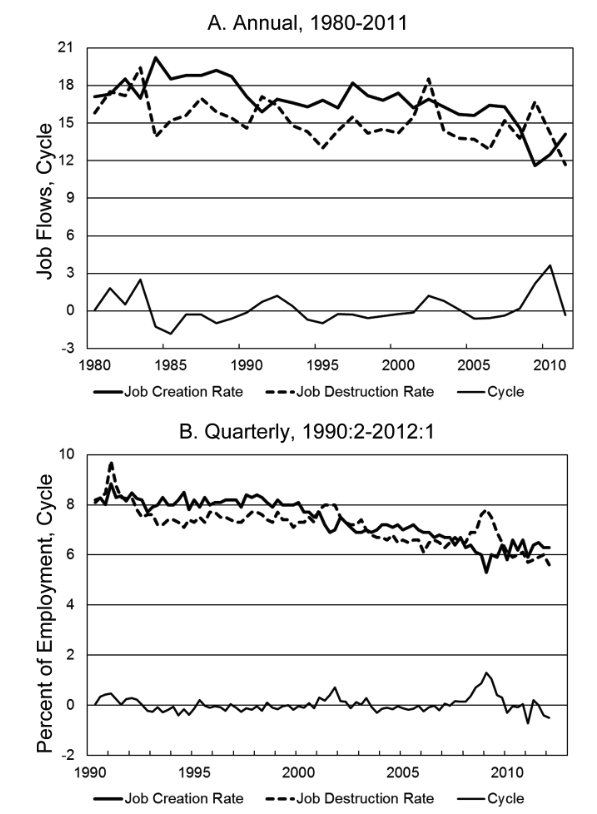
\includegraphics[scale = 0.6]{Plot1.1.png}
    \caption{Figure Job flows and the business cycle. Authors' calculations using Business
    Dynamics Statistics (annual), Business Employment Dynamics (quarterly), and
    the Current Population Survey. Cycle is the change in the unemployment rate.
    }
    \label{plot:1.1}
\end{figure}
The graph also depicts the fluctuations in the unemployment rate, clearly demonstrating that periods of rising
unemployment are typically marked by increased job losses and decreased job creation. However, the trend took a notable
turn during the Great Recession. Specifically, while job losses did surge in the 2008-2009 period, the most remarkable
change was the significant drop in job creation beginning in 2007 and extending through 2010. Additionally, there is an
observable long-term decline in job flow dynamics, a topic for further discussion. 

To corroborate these findings and delve into more granular data, they utilized the Business Employment Dynamics (BED)
statistics for the U.S. private sector. The BED's quarterly data from the second quarter of 1990 to the first quarter of
2012 (Panel B of the figure) underscores the annual trends, showing that recessions typically involve higher job
destruction and lower job creation rates. The period starting in 2007 stands out for a particularly steep decline in job
creation, a trend that is more pronounced in the BED data. The BED series also highlights that the sluggish recovery
from the Great Recession up to early 2012 is primarily attributable to weak job creation rather than enduringly high job
destruction rates. This pattern, confirmed by other datasets such as the Job Openings and Labor Turnover Survey (JOLTS),
persisted beyond the first quarter of 2012. 

Adding to this, job creation during the Great Recession was as low as it has been at any time in the past 30 years, as
illustrated in the figure. Moreover, job reallocation (the sum of job creation and destruction) reached its lowest point
in 30 years during the Great Recession and its immediate aftermath. When comparing the Great Recession to the early
1980s recession, the rate of job reallocation was 28\% in 2009, in stark contrast to 35\% in 1983 (both periods represent
peaks in job destruction and are measured using March-to-March Business Dynamics Statistics data). These patterns are
partly driven by significant downward trends in job flows, as evidenced in both the Business Dynamics Statistics (BDS)
and the BED data. Although exploring the causes of these declining trends in job flows is beyond the scope of this
analysis, it is clear that these trends are significant and have been taken into account in the analysis. 

Moreover the authors show how the patterns change considerbaly in the great recession, in particularly regarding how the
creation and distruction rate og jobs respond to the sharp fall in demand. They found as expected from \cite{CabHarm94}
that the creation rate of new jobs slower before the crisis spread out and than the distruction rate increses when it is
not possible to fully accommodate the decrease in demand only stopping new labour hiring. They asses that during the
Great Recession this patterns changes in particularly the fraction of net employment  contraction accounted by a job
reduction is higeger than 0.5, while for all the previous recession it was way below 0.4 as shown in the table.
\begin{table}[ht]
    \centering
    \caption{
    Share of Change in Net Employment Growth Due to Change in Job Creation in Periods of Net Contraction}

    \begin{tabular}{lccc}
    \hline & \multicolumn{2}{c}{ National } & State \\
    \cline { 2 - 3 } Period & BDS (Annual) & BED (Quarterly) & BDS (Annual) \\
    \hline Pre-Great Recession & .21 & .28 & .39 \\
    Post-2007 & .61 & .59 & .65 \\
    \hline
    \end{tabular}
    \label{tab:1.2}
\end{table}

This analysis is based on the authors' computations using data from the Business Dynamics Statistics (BDS) and Business
Employment Dynamics (BED). The methodology hinges on the principle that net employment change equals job creation minus
job destruction. For any period(s) of net employment decrease lasting at least one period, both the total change in net
employment growth and the total change in job creation are aggregated over the full duration of consecutive net
contraction periods. Furthermore, these aggregated changes are then further combined within the periods outlined in the
analysis. The proportion mentioned refers to the fraction of the total aggregated change in net employment growth during
the specified timeframe that is attributed to the total change in job creation within the same timeframe. Specifically,
the BDS data spans from 1981 to 2007 for the pre-Great Recession era and from 2008 to 2011 for the post-2007 era. For
the BED, the pre-Great Recession period covers from the second quarter of 1990 to the third quarter of 2007, and the
post-2007 era from the fourth quarter of 2007 to the first quarter of 2012. It's important to note that these
calculations are applied solely to periods experiencing a net decrease in employment growth. For instance, this applies
to the period from the fourth quarter of 2007 to the first quarter of 2010 for the BED data. Regarding the BDS National
Annual data, there are six years of net employment contraction, with two of those years occurring after 2007. In the BED
Quarterly data, there are twenty-two quarters of net contraction, with nine quarters following 2008. For the BDS State
Annual data, there are 393 state-year instances of net contraction, with 112 of those instances occurring after 2007. 

Another way to see this change in patterns is regressing job creation rate, job destruction rate and Reallocation rate
to Cyle an iteration between a Great Recession dummy and the cycle and a trend. The results are shown in the table 3.
\begin{table}
    \centering
    \caption{Job Flows and Change in the Unemployment Rate at the State-Level (Annual), 1981-2011}
    \begin{tabular}{|c|c|c|c|}
    \hline & \begin{tabular}{l} 
    Job Creation \\
    Rate
    \end{tabular} & \begin{tabular}{c} 
    Job Destruction \\
    Rate
    \end{tabular} & Reallocation Rate \\
    \hline Cycle & \begin{tabular}{l}
    $-.631 ***$ \\
    $(.046)$
    \end{tabular} & \begin{tabular}{l}
    $1.194 ***$ \\
    $(.053)$
    \end{tabular} & \begin{tabular}{l}
    $.563 ***$ \\
    $(.068)$
    \end{tabular} \\
    \hline GR $\times$ cycle & \begin{tabular}{l}
    $-.371 ***$ \\
    $(.079)$
    \end{tabular} & \begin{tabular}{l}
    $-.421^***$ \\
    $(.079)$
    \end{tabular} & \begin{tabular}{l}
    $-.793 ***$ \\
    $(.128)$
    \end{tabular} \\
    \hline Trend & \begin{tabular}{l}
    $-.168***$ \\
    $(.010)$
    \end{tabular} & \begin{tabular}{l}
    $-.136 ***$ \\
    $(.011)$
    \end{tabular} & \begin{tabular}{l}
    $-.304***$ \\
    $(.020)$
    \end{tabular} \\
    \hline
    \end{tabular}
    \footnote{$-N=1,581$. GR is a dummy variable equal to one for years from 2008 to 2010 (job flows from March 2007 to March 2010). Cycle is the state-year change in the unemployment rate. All specifications include state fixed effects. Standard errors in parentheses are clustered at the state level.
    $$
     because * \quad p<.01 \text {. }
    $$}
    \label{tab:1.2}
\end{table}
The authors delve into the nuances of state-level job flow dynamics by leveraging the variation in the relationship
between cyclical economic indicators and job flows across different states. Their methodological approach is rooted in
conducting descriptive regressions that not only link job flows to a selected cyclical indicator but also incorporate an
interaction term that captures the distinctive economic conditions of the Great Recession period alongside the cyclical
variable. To achieve this, they meticulously utilize changes in the unemployment rate at the state level as a proxy for
economic cycles. Recognizing the persistent negative trend in job flows across the board, the authors judiciously
incorporate a linear trend into their regression models to adequately account for this overarching pattern. 

The findings from these regressions are illuminating, revealing that cyclical fluctuations predominantly explain a
substantial portion of the variance observed in job flows, particularly with respect to the job destruction rate. This
observation is in line with the theoretical framework posited by \cite{CabHarm94}, which suggests that the
margin of job destruction exhibits a higher sensitivity to cyclical downturns compared to the job creation margin. A
striking aspect of their analysis is the significant and negative interaction observed between the cyclical variable and
the Great Recession dummy variable, indicating that this period was characterized by a pronounced decrease in the rate
of new job openings, whereas the rate of job layoffs was not as severely affected as it had been in other recessions.
This pattern underscores the profound and distinctive impact of the Great Recession, which led to a dramatic downturn in
job creation, surpassing the declines observed in job destruction rates and deviating markedly from the trends seen in
prior economic downturns. 

Furthermore, the analysis sheds light on the behavior of the job reallocation rate during the Great Recession, which, in
a departure from its traditionally pro-cyclical nature observed in earlier recessions, switched signs, indicating a
contraction in job reallocation. This reversal is particularly noteworthy as it signifies a shift towards less job
reallocation, thereby challenging the conventional understanding of job flow dynamics during economic downturns. 

An important contribution to this discourse comes from studies that emphasize the significant role of young businesses
in the observed decline in job creation rates, particularly highlighted in the research by \cite{fort2013firms}. These young
businesses, defined as entities with less than five years of operation, exhibit a markedly higher responsiveness in
their job creation margin, especially in the aftermath of the 2007 financial crisis. This responsiveness is contrasted
with the behavior of older firms, which, although also experiencing shifts in their job creation and destruction
margins, do not demonstrate the same level of sensitivity as their younger counterparts. The distinction between young
and old firms becomes even more pronounced when examining the destruction margin, where young firms again show a greater
responsiveness, underscoring the differential impact of economic cycles based on firm age. 

The second question that the authors try to adress was: Did Cleansing Effect change in the great recession?
In order to adress this question the authors focus on analysis if th
\begin{figure}
    \centering
    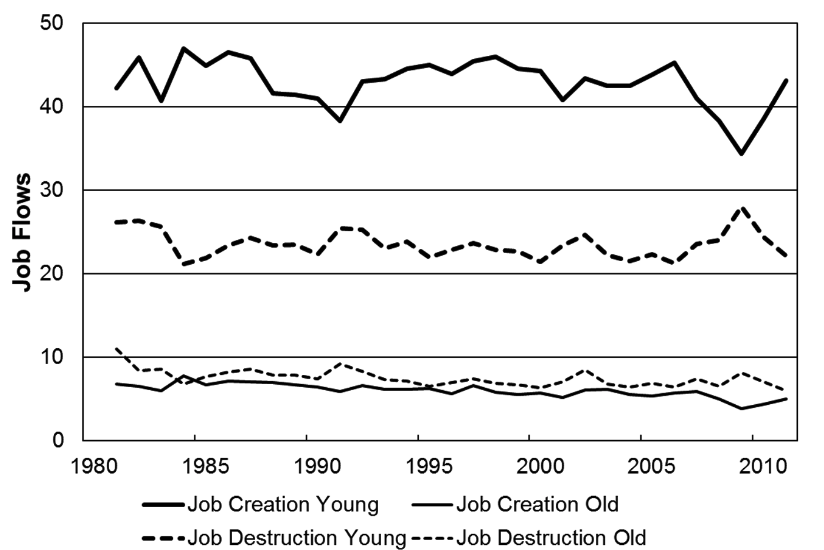
\includegraphics[scale = 0.54]{Plot1.2.png}
    \caption{Job flows by age, 1981-2011. Authors' calculations on Business Dy-
    namics Statistics. Young is for establishments owned by firms less than 5 years old.
    Mature is for establishments owned by firms 5 or more years old. Job flows are
    establishment based and are classified by firm age characteristics.
    }
    \label{plot:1.1}
\end{figure} 
\section{\cite{OsePap17}}
The economy comprises risk-neutral firms with a constant discount rate represented by $0 < \beta < 1$. These firms
exhibit heterogeneity in productivity and net worth. They employ a production technology that relies solely on capital
(or production units) as input, featuring diminishing returns to scale.
\\
In each period, firms incur a fixed production cost denoted as $c$ to initiate production. After production, they decide
how to allocate profits for the next period. The remaining profits are invested in a risk-free asset. Firms face a
choice: they can either continue operating and reinvest their profits or exit the market, investing their entire net
worth, denoted as $e$, in the risk-free asset.
\\
Firms opt to exit the market when expected profits no longer outweigh the fixed cost $c$, or when the value of
production becomes inferior to the value they could gain by investing in the risk-free asset.
\\
The value obtained from investing in the risk-free asset is given by:
\[
q_t + \sum_{s=0}^{+\infty}\beta^s[\beta(1+r)-1]e_{t+s+1}.
\]

Notably, when the condition $\beta(1+r) \leq 1$ holds, this value simplifies to $q$. In such cases, firms are either
indifferent regarding the timing of dividend distributions or have a preference for distributing their end-of-period net
worth to shareholders or investors.
\\
In this economic model, the agents are the firms themselves, aiming to maximize their value over time by selecting an
optimal level of capital denoted as $k$. The production function, accounting for the fixed cost $c$, is expressed as
follows: $Y = Z(\theta + \epsilon)k^\alpha$.
\\
Key variables include:
\begin{itemize}
    \item $Z$: Stochastic aggregate productivity common across firms.
    \item $\theta$: Persistent firm-specific productivity shock (modeled as a Markov Chain).
    \item $\epsilon$: Firm-specific productivity shock with $\epsilon \sim \mathcal{N}(0,\delta)$.
    \item $k^\alpha$: Capital or production units, as in Caballero and Hammour (AER).
\end{itemize}

The timeline of events is as follows:

\begin{figure}[h]
    \centering
    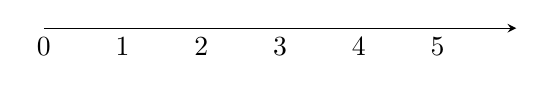
\begin{tikzpicture}
        % Draw timeline
        \draw[->,>=stealth] (0,0) -- (6,0);
        
        % Add timeline labels
        \foreach \x/\label in {0,1, 2,3, 4, 5} {
            \node[align=center, below] at (\x,0) {\label};
        }
    \end{tikzpicture}
    \caption{Timeline of Events}
\end{figure}

The sequence of events includes:
\begin{enumerate}
    \item The firm possesses knowledge of $Z,\theta,k^\alpha,e$ (where $e$ represents its endowment, different from $k$ since the firm can borrow money with $d=c+k-e$).
    \item The firm computes the optimal $k$ to maximize the expected value of the firm, with $k$ ranging from $[0,+\infty]$. If $k=0$, it indicates the firm's decision to exit.
    \item At the end of the period, the firm observes $\epsilon$ and the aggregate shock.
    \item The firm repays its debt and the fixed operating cost $(c+k-e)$, resulting in an end-of-period net worth $q$.
    \item The firm decides on the amount of dividends to distribute $(q-e')$, observes the productivity shock $\theta', Z'$, and the process restarts from step 1.
\end{enumerate}

\subsection{Frictionless economy}
In a frictionless economy, firms have the option to borrow an amount denoted as \(c+k-e\) at the risk-free interest rate
\(r=\frac{1}{\beta}-1\). Therefore, at the start of the period, the firm's value is determined by the following
expression:

\[V_{FL} = \max_{k} E \int \max[q,\max_{e'}(q - e' + \beta V_{FL}(e',\theta', Z'))]  \,d\Phi
(\epsilon) \]
where the end of period net worth is equal to:
\[q=Z(\theta+\epsilon)k^\alpha + (1-\delta )k-(1+r)(c+k-e)\]

Under the condition of survival, it can be demonstrated that:

\[\widehat{V}_{FL}(\theta,Z) = \max_{k}E\int[Z(\theta+\epsilon)k^\alpha - (1+r)c\,d\Phi (\epsilon)] +
\beta\max[0,\widehat{V}_{FL}(\theta',Z')]\]

In the absence of market frictions, firms choose to exit when their productivity reaches a certain threshold.
Specifically, they exit if \(\theta'<\underline{\theta} _{FL}(Z')\), where \(\underline{\theta}
_{FL}(Z')\) is defined as the value
for which \(\widehat{V}_{FL}(\underline{\theta}_{FL},Z')=0\).

\subsection{Economy with Credit Market Frictions}

After production, the firm privately observes the temporary shock $\epsilon$, while financial intermediaries can only
observe it at a cost of $\mu k^\alpha$. For one-period debt contracts, financial intermediaries observe $\epsilon$ only
if the firm faces financial distress, which occurs when the private shock is insufficient to repay its debt. The terms
of the financial contract depend on the firm's net worth $e$, current productivity $\theta$, and aggregate productivity
value $Z$, all observable by both the financial intermediary and the firm at no additional cost.

\textbf{HP1 (Hypothesis 1):} The risk-free interest rate is $\beta < \frac{1}{1+r}$, which implies a lower risk-free
rate in an economy with credit frictions compared to a frictionless one. It also ensures that firms do not always
reinvest their profits.

When a firm defaults, the financial intermediary incurs verification costs and seizes all of the firm's income. The
default threshold $\overline{\epsilon}$ is determined by the equation:
\[
Z(\theta+\overline{\epsilon})k^\alpha + (1-\delta)k = (1+\widetilde{r} )(c+k+e)
\]

Default results in a zero net worth but does not necessarily force the firm to exit the market, depending on its
persistent productivity component $\theta$.

The financial intermediary lends $(c + k - e)$ to the firm only if the expected income from the loan equals the
opportunity cost of the funds, as expressed by the inequality:
\[
(1+\widetilde{r} )(k+c+e)(1-\Phi(\overline{\epsilon}))+\int_{-\infty}^{\overline{\epsilon}}[Z(\theta+\overline{\epsilon})
k^\alpha+(1-\delta)k-\mu k^\alpha] \,d\Phi(\epsilon) \geq (1+r)(c+k+e)
\]

The financial contract is characterized by $(k,\overline{\epsilon})$. Given $Z,\theta,e$, the participation constraint
indicates the default threshold $\overline{\epsilon}$ required by the financial intermediary to lend a given amount. For
some firms, their net worth is too low for the participation constraint of the financial intermediary to be satisfied.
In fact, given $\theta, Z$, there is a unique threshold $e_b(\theta,Z)$ below which the financial intermediary
refuses to lend any amount:
\[
Z[\theta+G(\overline{\epsilon}_b )]k^\alpha+(1-\delta)k-uk_b^\alpha\Phi (\overline{\epsilon}_b)=(1+r)(k_b+c-\underline{e_b})
\]
where $\overline{\epsilon}_b$ maximizes the expected income of the financial intermediary. When the firm has a net worth
below $\underline{e_b}$, the firm defaults.

After production, the firm's end-of-period net worth is equal to:
\[
q = \begin{cases}
  Z(\theta+\overline{\epsilon})k^\alpha +(1-\delta)k-(1+\widetilde{r})(k+c-e) & \text{if } \epsilon\geq \overline{\epsilon} \\
  0 & \text{otherwise}
\end{cases}
\]
Using the default condition we can rewrite as 
\[q = \max[Zk^\alpha(\epsilon-\overline{\epsilon});0]\]

\subsection{The firm's problem}
Define $V$ as the firm's value at the start of the period, which hinges on investment outcomes and exit decisions. If
the end-of-period net worth falls below a threshold ($q < e_b(\theta', Z')$), the firm exits. Otherwise, it compares its
continuing value to the end-of-period net worth ($q \geq e_b(\theta', Z')$) and exits if the continuing value is lower.

The firm's value function is given by:
\[
V(e,\theta,Z) = \max_{(k,\overline{\epsilon})}E\left\{\int I(q)q + (1-I(q))\max[q,\max_{e'}q-e'+\beta V(e',\theta',
\zeta')]\,d\Phi(\epsilon)\right\}
\]

Where:
\[
I(q)=
\begin{cases}
    0 & \text{if } q\geq e_b(\theta', Z')\\
    1 & \text{if } q< e_b(\theta', Z')
\end{cases}
\]

Subject to the following constraints:
\begin{enumerate}
    \item \label{con1}\[
    Z[\theta+G(\overline{\epsilon}_b )]k^\alpha+(1-\delta)k-uk_b^\alpha\Phi (\overline{\epsilon}_b)\geq(1+r)(k_b+c-
    \underline{e_b})
    \]
    \item \label{con2} \[
    q = \max[Zk^\alpha(\epsilon-\overline{\epsilon});0]
    \]
    \item \label{con3}\[
    \overline{e_b}(\theta',Z)\leq e'\leq q
    \]
\end{enumerate}

The firm aims to maximize expected dividends while complying with the financial intermediary's participation constraint
(constraint 1). Equation (constraint 2) characterizes the firm's end-of-period net worth, and
Equation (constraint 3) ensures that the
net worth
is sufficiently high to satisfy the participation constraint.
\par
Furthermore, the firm is prohibited from issuing new shares and can only augment its net worth by reinvesting profits.
This limitation presents a trade-off: increasing capital boosts production capacity but also raises the risk of default,
as the default threshold set by the financial intermediary increases with borrowed amounts.
\section{The cleansing effect by Caballero}
\subsection{Introduction}
In the first paper that rationalize the cleansing effect of recessions, authored by Ricardo J. Caballero and Mohamad L.
Hammour  \cite{CabHarm94} and published in the American Economic Review in 1998, the primary aim was to investigate how
industries respond to cyclical variations in demand. They did this by employing a vintage model of creative destruction.
The underlying concept postulates that the processes of creation and destruction within an industry partially explain
business cycles. Industries continuously experiencing creative destruction can adapt to demand fluctuations in two
ways: by adjusting the rate at which they produce new units embodying advanced techniques or by altering the
rate at which outdated units are retired. The model they used incorporated heterogeneous firms, where production units
embodied the most advanced technology at the time of their creation. The costs associated with creating new units
slowed down technology adoption, resulting in the coexistence of production units with varying vintages.
\par
Key to understanding how firms adapt to business cycles are the concepts of the creative margin and the destruction
margin. For example, a reduction in demand can be accommodated either by reducing the rate of technology adoption or by
retiring older production units. One of the primary factors determining which margin is more responsive to business
cycles is the adjustment cost. When this cost follows a linear pattern, the study shows that insulation is complete, and
the industry's response relies exclusively on its creation margin. Consequently, the creation margin becomes smoother
over time in comparison to the destruction margin, which exhibits greater responsiveness to the business cycle.
\par
Crucially, Caballero and Hammour's research \cite{BlaDia90} offers theoretical insights supported by empirical
evidence. Their findings on the cyclical nature of the destruction margin align with the studies conducted by Blanchard
and Diamond \cite{BlaDia90}, as well as Steven Davis and John Haltiwanger \cite{DavHalt92}, in their respective works
from 1990. This
convergence between theoretical framework and empirical substantiation underscores the importance of comprehending the
dynamic interplay between creative destruction and business cycles, which significantly influences how industries
respond to economic fluctuations.
\par
In their study \cite{DavHalt92}, where they assess the heterogeneity of employment changes at the establishment level in
the U.S. manufacturing sector from 1972 to 1986, it is revealed that job destruction exhibits procyclical tendencies,
responding more robustly to downturns in the economic cycle compared to the creation rate, in line with the theoretical
model proposed by Caballero and Hammour \cite{CabHarm94}. The authors leverage a natural experiment inherent in the data
to examine whether the structure of adjustment costs can account for the behavior of these two margins. This natural
experiment arises from the asymmetric nature of business cycles, with recessions being shorter but more severe than
expansions. The theoretical model predicts that these differences should be attenuated in the creation process, a
prediction that is substantiated by the data since creation exhibits relative symmetry around its mean, while
destruction displays a high degree of asymmetry.
The underlying concept driving the behavior of the destruction margin can be traced back to the theories of Schumpeter
and Hayek.  They suggest that recessions represent periods during which unprofitable or outdated techniques are pruned
from the economy, leaving behind the most efficient firms \citet{HaCa07}.
\subsection{Theoretical model}
The model in question is a vintage model that simulates an industry experiencing exogenous technological progress.
Within this model, production units are constructed using a fixed proportion of labor and capital, and they are
continually being created and phased out. Notice that only the creation of new production units
incurs a cost. This simplification is plausible, particularly in the context of the United States, where the expense
associated with hiring is typically higher than the cost of termination, as demonstrated by Abdulkadiroğlu and Kranton
(2003) \cite{AbdKra03}. 
\par
In this model, when a production unit is created at a specific time \(t_0\), it embodies the most advanced technology
available at that moment and consistently generates a uniform output represented by \(A(t_0)\) throughout its
operational lifetime. The productivity of this technology, denoted as \(A(t)\), experiences continuous growth at an
exogenously determined constant rate \(\delta \ge 0 \). This growth in technology can be interpreted in two ways: either
as the adoption of new technology or as a product innovation. In the latter scenario, a continuum of perfectly
substitutable products can yield varying levels of output.

\[\left[ f(a,t) \qquad 0\leq a \leq \overline{a}(t) \right]\]

The above function represents the cross-sectional density of the production units aged \(a\) at time \(t\), where
\(\overline{a}(t)\) is the age of the oldest production unit at time \(t\). The first assumption is that \(f(a,t)\) and
\(\overline{a}(t)\) are continuous functions. The mass of production units at time \(t\) is given by:

\[N(t) = \int_{\overline{a}(t)}^{0}f(a,t)da\]

\(N(t)\) is a measure of either the industry's capital stock and its employment, due to a fixed share of capital and
labor. Thus, the industry's output is given by:

\[Q(t) = \int_{\overline{a}(t)}^{0}A(t-a)f(a,t)da\]

The deterioration of production units involves both an exogenous depreciation rate \(\delta\) and an endogenous
destruction process, which impacts \(f(a,t)\) at its limits. The count of production units surviving for \(a\) years is
expressed as: 

\[f(a,t)= f(0,t-a)e^{-\delta a} \quad \text{where } 0 < a \leq \overline{a}(t)\]

The production flow is determined by:

\[\dot{N}(t) = f(0,t) [1-\overline{\dot{a}}(t)] + \delta N(t)\]

Here, the first term represents the production rate, while the second term encapsulates the destruction rate,
encompassing the obsolescence rate \(f(\overline{a})(t)\), the technological obsolescence change over time
\(-f(\overline{a})(t)\overline{\dot{a}}(t)\), and the depreciation rate \(\delta N(t)\). 

The assumptions made by the authors are denoted as \(\forall t \mid f(0,t)>0 \cup  \overline{\dot{a}}(t)<\).

The alteration in output concerning these flows is articulated as:

\[\dot{Q}(t) = A(t)f(0,t) - A(t-\overline{a}(t))f(\overline{a}(t),t) \cdot [1-\overline{\dot{a}}(t)] + \delta Q(t)\]

The authors define a perfectly competitive industry in partial equilibrium, where supply is dictated by free entry and
perfect equilibrium. Additionally, they introduce a cost function related to creating new production units: 

\[c = c\left(f\left(f(0,t)\right)\right) \quad \text{where } c(\cdot)>0, \, c'(\cdot)\leq 0\]

This cost function is contingent on the creation rate, implying that higher creation rates correspond to increased
costs. The equilibrium condition is established by equating the cost of unit creation to the present discounted value of
profits throughout its lifespan. The authors set the cost of a production unit to 1, and \(P(t)\) is the price of a unit
of output. Thus, the profits generated at time \(t\) by a production unit aged \(a\) are defined as: 

\[\pi(a,t)= P(t)A(t-a)-1\]
\[\overline{a}[t+T(t)] = T(t)\]

Here, \(T(t)\) signifies the maximum lfetime of a unit created at \(t\). At any given time \(t\), the free entry
condition is expressed as: 

\[ c(f(0,t)) = \int_{t+T(t)}^{t}\pi(s-t,t)e^{-(r+\delta)(s-t)\,ds} \]

In the above equation, where \(r>0\) represents the exogenously determined instantaneous interest rate, the determination of
the exit of a production unit is contingent upon continuous \(P(t)\) and the instance when the profits generated by a
unit being destroyed reach zero. This occurrence signifies the moment when the oldest unit operational at time \(t\),
denoted as \(\overline{a(t)}\), must adhere to the equation: 

\[P(t)A(t-\overline{a}(t))=1\]

The authors posit that \(P(t)\) exhibits a decreasing trend due to the model's assumption regarding endogenous
destruction, specifically \(\overline{\dot{a}(t)}<1\). To see, differentiate 
\[\dot{P}(t)=-\gamma\left[1-\overline{\dot{a}}P(t)\right]\]
Consequently, when the profits of a production unit diminish to
zero for the first time, it will be subject to destruction. 

On the demand side, the authors assume a unit-elastic demand function and consider the aggregate expenditure as
exogenous 
\(\overline{D}(t)=P(t)Q(t)\). 
The equilibrium is a path \(\left\{f(0,t),\overline{a}(t),T(t),Q(t)\right\}_{t \geq 0}\) that satisfy the following
conditions:
\begin{enumerate}
    \item \label{eq_2.1} $ \begin{aligned}[t]
        Q(t) &= \int_{\overline{a}(t)}^{0}A(t-a)f(a,t)da
    \end{aligned}$
    \item \label{eq_2.2}$ \begin{aligned}[t]
        f(a,t)&=f(0,t-a)e^{-\delta a}      
    \end{aligned}$
    \item \label{eq_2.3}$ \begin{aligned}[t]
        T(t)&=\overline{a}\left(t+T(t)\right)        
    \end{aligned}$
    \item \label{eq_2.4}$ \begin{aligned}[t]
        c(f(0,t))&=\int_{t}^{t+T(t)}\left[P(s)A(t)-1\right]e^{-(r+\delta)(s-t)}\,ds
    \end{aligned}$
    \item \label{eq_2.5}$ \begin{aligned}[t]
        P(t)A(t-\overline{a}(t)=1)
    \end{aligned}$
    \item \label{eq_2.6}$ \begin{aligned}[t]
        P(t)Q(t)=\overline{D}(t)
    \end{aligned}$
\end{enumerate}
The first three equations (\ref{eq_2.1}, \ref{eq_2.2}, \ref{eq_2.3}) and the fifth one (\ref{eq_2.5}) suffice to
delineate the trajectories of \(T(t)\), \(P(t)\), and \(Q(t)\), which are determined by \(\left\{f(0,t),
\overline{a}(t)\right\}\). To affirm the robustness of the conditions expressed in equations \ref{eq_2.6} and
\ref{eq_2.5}, it is possible to derive these equations as first-order conditions for the maximization of a number of
perfectly competitive firms holding production units. 

To comprehend the functioning of endogenous destruction, let's consider a scenario with constant demand. In this case,
both the destruction and creation rates change only due to supply factors. This steady state is characterized by a
constant lifetime of production units \(T(t) = \overline{a}(t) = \overline{a}^*\), resulting in a time-invariant age
distribution \(f(a,t) = f^*(a)\). Equation \ref{eq_2.5} implies that the price \(P(t)\) must consistently decrease at a
rate \(\sigma\). Higher innovation rates lead to increased productivity, raising the supply and consequently lowering
the price. Equation \ref{eq_2.2} reveals that the distribution of production units in the steady state follows a
truncated exponential distribution: 

\[f^*(a) = f^*(0)e^{-\delta a} \quad 0 \leq a \leq \overline{a}^*\]

Using free entry conditions (\ref{eq_2.4}) and the clearing condition (\ref{eq_2.6}), one can determine the creation and
destruction ages \(f^*(0)\) and \(\overline{a}^*\). Equations \ref{eq_2.1} and \ref{eq_2.5} yield the cost function and
productivity of a new production unit: 

\[\label{eq_2.7} c(f^*(0)) = \frac{e^{\gamma \overline{a}^*} - e^{-(r + \delta)\overline{a}^*}}{\gamma + r + \sigma} - \frac{1 - e^{-(r + \delta)\overline{a}^*}}{r + \delta}\]

\[\label{eq_2.8} f(0) = \frac{(\sigma + \delta)\overline{D}^*}{e^{\sigma \overline{a}^* - e^{\delta \overline{a}^*}}}\]

The authors then normalize the creation rate:

\[N = f^*(0) \cdot (1 - e^{\delta \overline{a}^*})\]

In the steady state, this is given by:

\[(9) \label{eq2.9}CC^* = \frac{\delta}{1 - e^{-\delta \overline{a}^*}}\]

Considering a special case where the creation cost is a constant \(c\), i.e., \(c(f^*(0)) = c\), substituting into
equation \ref{eq_2.7} allows retrieval of \(\overline{a}^*\). The effect of technological rate \(\sigma\) on
\(\overline{a}^*\) is decreasing, as a higher innovation rate increases the opportunity cost of delayed renovation,
while a higher cost of creating new units lowers the renovation rate. Optimal lifetime of production units increases
with higher \(r\) and \(\delta\) as it becomes harder to recover creation costs. 

Now, dropping the assumption of constant demand, we examine how the industry adjusts to demand fluctuations. Two ways
are identified in which the industry adapts production to meet demand: by reducing the rate of creation \(f(0,t)\) and
by increasing the rate of endogenous destruction \(f(\overline{a}(t),t) \cdot [1-\overline{\dot{a}}(t)]\), thus reducing
\(\overline{a}\), the age at which units are demolished. 

These two adjustments interact, leading to a reduction in demand causing the most outdated units to be scrapped,
rendering them unprofitable. However, if the recession is partially accommodated by a reduction in the creation rate,
the effect on the destruction margin is diminished. The authors argue that the extent to which creation will "insulate"
existing units from variations in demand depends on the marginal cost of creating new units \(c'f(0,t)\). When the
marginal cost of creation is zero, demand fluctuations are entirely adjusted by the creation margin. This is exemplified
in the case where \(c(f(0,t)) = c\). In such instances, the insulation effect is complete, as there is no need to retire
older units. Lowering \(f(0,t)\) is sufficient, and it is cheaper than reducing the life of existing production units. 

The insulation effect is not solely due to asymmetric adjustment costs on the creation and destruction margins. Complete
insulation would occur even with linear adjusting costs. The creation rate in the case of constant creation cost is
given by: 

\[\label{eq_2.10} f(0, t) = \frac{\dot{\bar{D}}(t) + \delta \bar{D}(t) + P(t) A(t - \bar{a}(t)) f(\bar{a}(t), t)[1 -
\dot{\bar{a}}(t)] - \dot{P}(t) Q(t)}{P(t) A(t)}\] 

In the attained equilibrium, variations in demand are entirely offset by adjustments at the creation margin denoted as
\(f(0, t)\), with \(\overline{a}(t)\) remaining steady at the destruction margin. The creation process effectively
counteracts the impact of demand fluctuations on the price \(P(t)\), effectively shielding existing units from demand
changes. The price \(P(t)\) experiences a constant decline at a rate represented by \(\sigma\), reflecting the pace of
technical progress. This consistent decline in \(P(t)\) serves as a clear signal for production units to function
optimally throughout their constant lifetime \(\overline{a}(t)^*\). \\
In the aforementioned scenario, the destruction rate is not constant, but it does not respond to demand through
variations in the age \(\overline{a}(t)^*\) at which units are destroyed. Instead, variations in the creation rates have
an impact on the number of units that reach obsolescence. If fewer units are created, fewer units become obsolete after
\(\overline{a}(t)^*\) periods. It is noteworthy that any modification leaving equations \ref{eq_2.3} to \ref{eq_2.5}
independent of \(\overline{D}(t)\) and \(f(0,t)\) does not alter the full-insulation results. 
\\
Interestingly, assumptions such as perfect competition, industry-wide return to scale, and perfect foresight are not
necessary for these conclusions. The latter is particularly noteworthy as it asserts that fully accommodating demand on
the creation side only requires knowledge of current conditions. As long as the non-negativity constraint on \(f(0,t)\)
is never binding, implementing equilibrium behaviors does not necessitate expectations of future demand. 
\subsection{Application of the model}
The model undergoes calibration utilizing Job-flow data and Industry production data. The former facilitates the
replication of job creation dynamics, while the latter is employed to mimic the behaviors of firm creation and
destruction in the manufacturing industry. To capture these dynamics, the marginal cost of creating new production units
is stipulated as positive \(c'f(0,t)\). This allows for a partial insulation effect, and the destruction margin responds
to demand fluctuations. However, introducing a dependency of \(c\) on \(f(0,t)\) compromises the analytical tractability
of the system (Equations \ref{eq_2.1} - \ref{eq_2.6}). Consequently, the authors resort to methods such as multiple
shooting to ascertain the optimal equilibrium and subsequently employ an iterative procedure to converge to the correct
expected creation rate. 

For numerical solutions, the authors adopt a linear formulation:

\[c(f(0,t))=c_0+c_1f(0,t)\]

To gain a deeper understanding of how creation and destruction respond to demand, the authors simulate sinusoidal demand
using the equation: 

\[\overline{D}(t)=1+0.07\sin(t)\]

The results are visualized in the image below, depicting the feedback of normalized creation and destruction (CC and DD)
to changes in demand. 

\begin{figure}
    \centering
    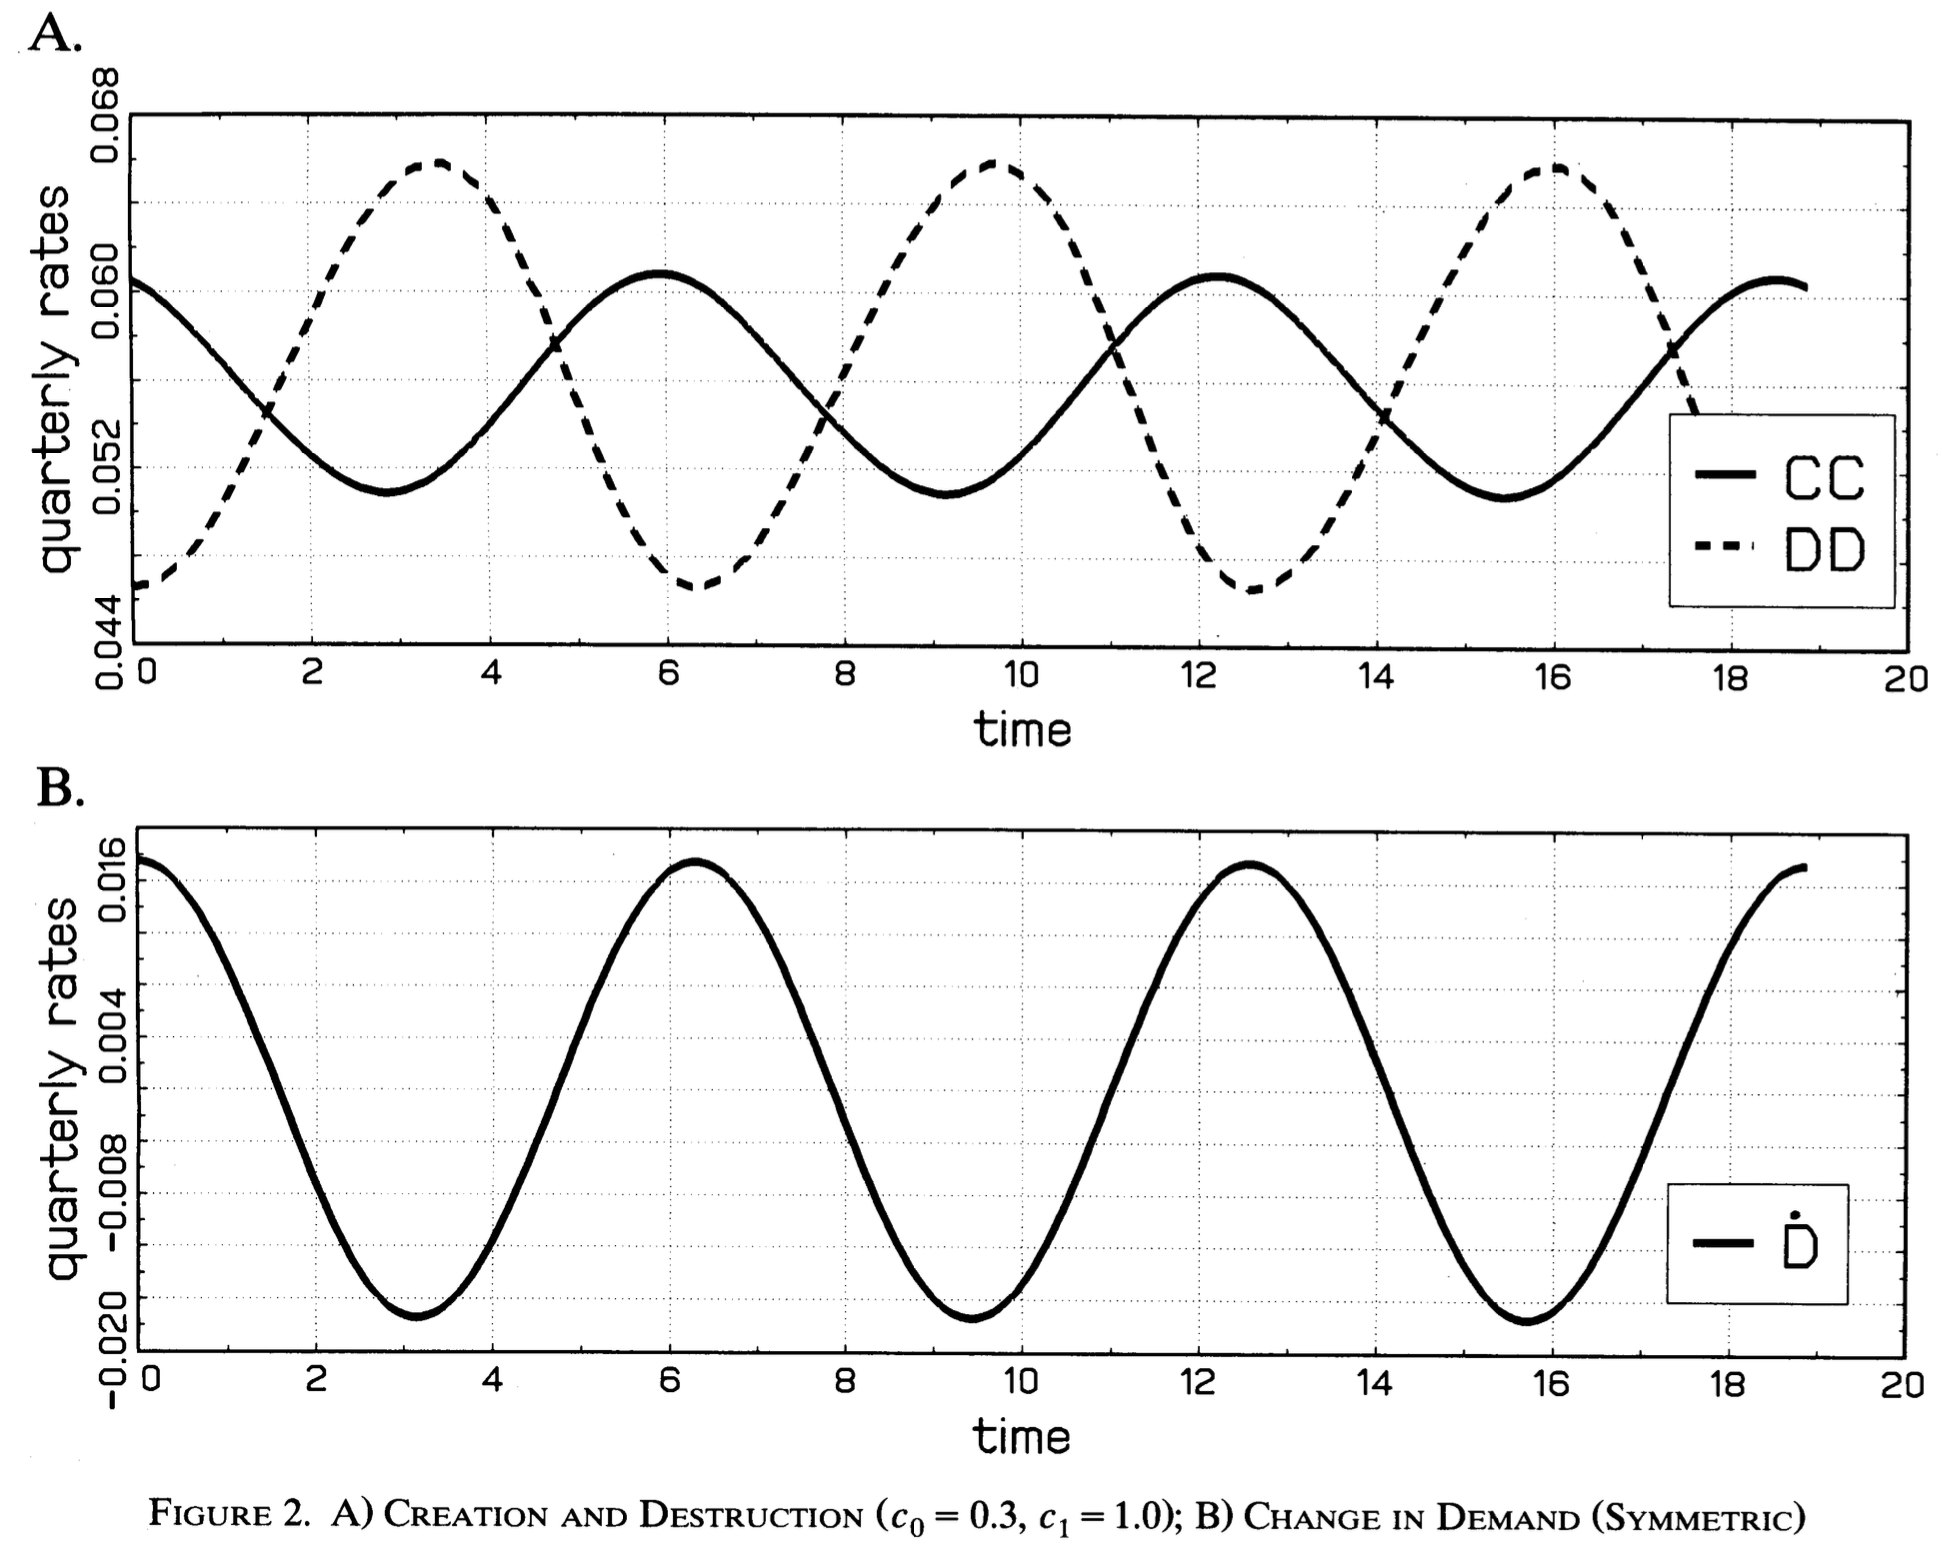
\includegraphics[scale = 0.4]{Plot2.1.png}
    \caption{Figure 1. A Creation and destruction \(c_0=0.3, c_1=1\) B Change in demand (Symmetric)}
    \label{plot:2.1}
\end{figure}

The plot clearly illustrates that the insulation effect is only partial; otherwise, DD would have remained flat, as in
the case with \(c(f(0,t)=c)\). From a mathematical perspective, destruction responds to demand as equations
\ref{eq_2.3}-\ref{eq_2.5} are no longer independent of the path \(f(0,t)\) and demand. From an economic standpoint,
increasing creation costs smoothen the creation process. In scenarios with a nearly flat innovation rate, firms during
crises cannot fully accommodate lower demand, nullifying the adoption of new production units, as the marginal costs
would exceed the reduction in existing production units. \par
In the considered model, production units integrate labor and capital in fixed proportions to generate output. Each unit
can be conceptualized as contributing to job creation within the industry, and job-flow data serves as a metric for
quantifying the flows of production units. 

Datasets that closely align with the theoretical CC and DD series have been compiled by Davis and Haltiwanger
\cite{DAvHalt90,DavHalt92} and Blanchard and Diamond \cite{BlaDia90}, drawing from various sources. The primary focus
lies on the dataset curated by Davis and Haltiwanger, who leverage the Longitudinal Research Database to construct
quarterly series for U.S. manufacturing plants spanning the period 1972:2-1986:4. 

In their empirical approach, \cite{DavHal94}utilize output to empirically determine demand, employing the growth
rate of the industrial production index as a proxy for output growth. Notably, in the foundational theoretical model,
\(Q(r)\) is smoothed by price movement, with the elasticity of demand determining the extent of smoothing, assumed to be
equal to 1. While the theoretical model maintains a constant consumption-wage, the authors acknowledge that considering
a procyclical consumption-wage, as in the case of general equilibrium with correlated industry shocks, may dampen the
effect of demand shocks. However, they assert that this adjustment would alter only the magnitude, not the direction, of
the analysis. 

The figure below illustrates the data that the model seeks to replicate, showcasing job creation, job destruction, and growth.

\begin{figure}
    \centering
    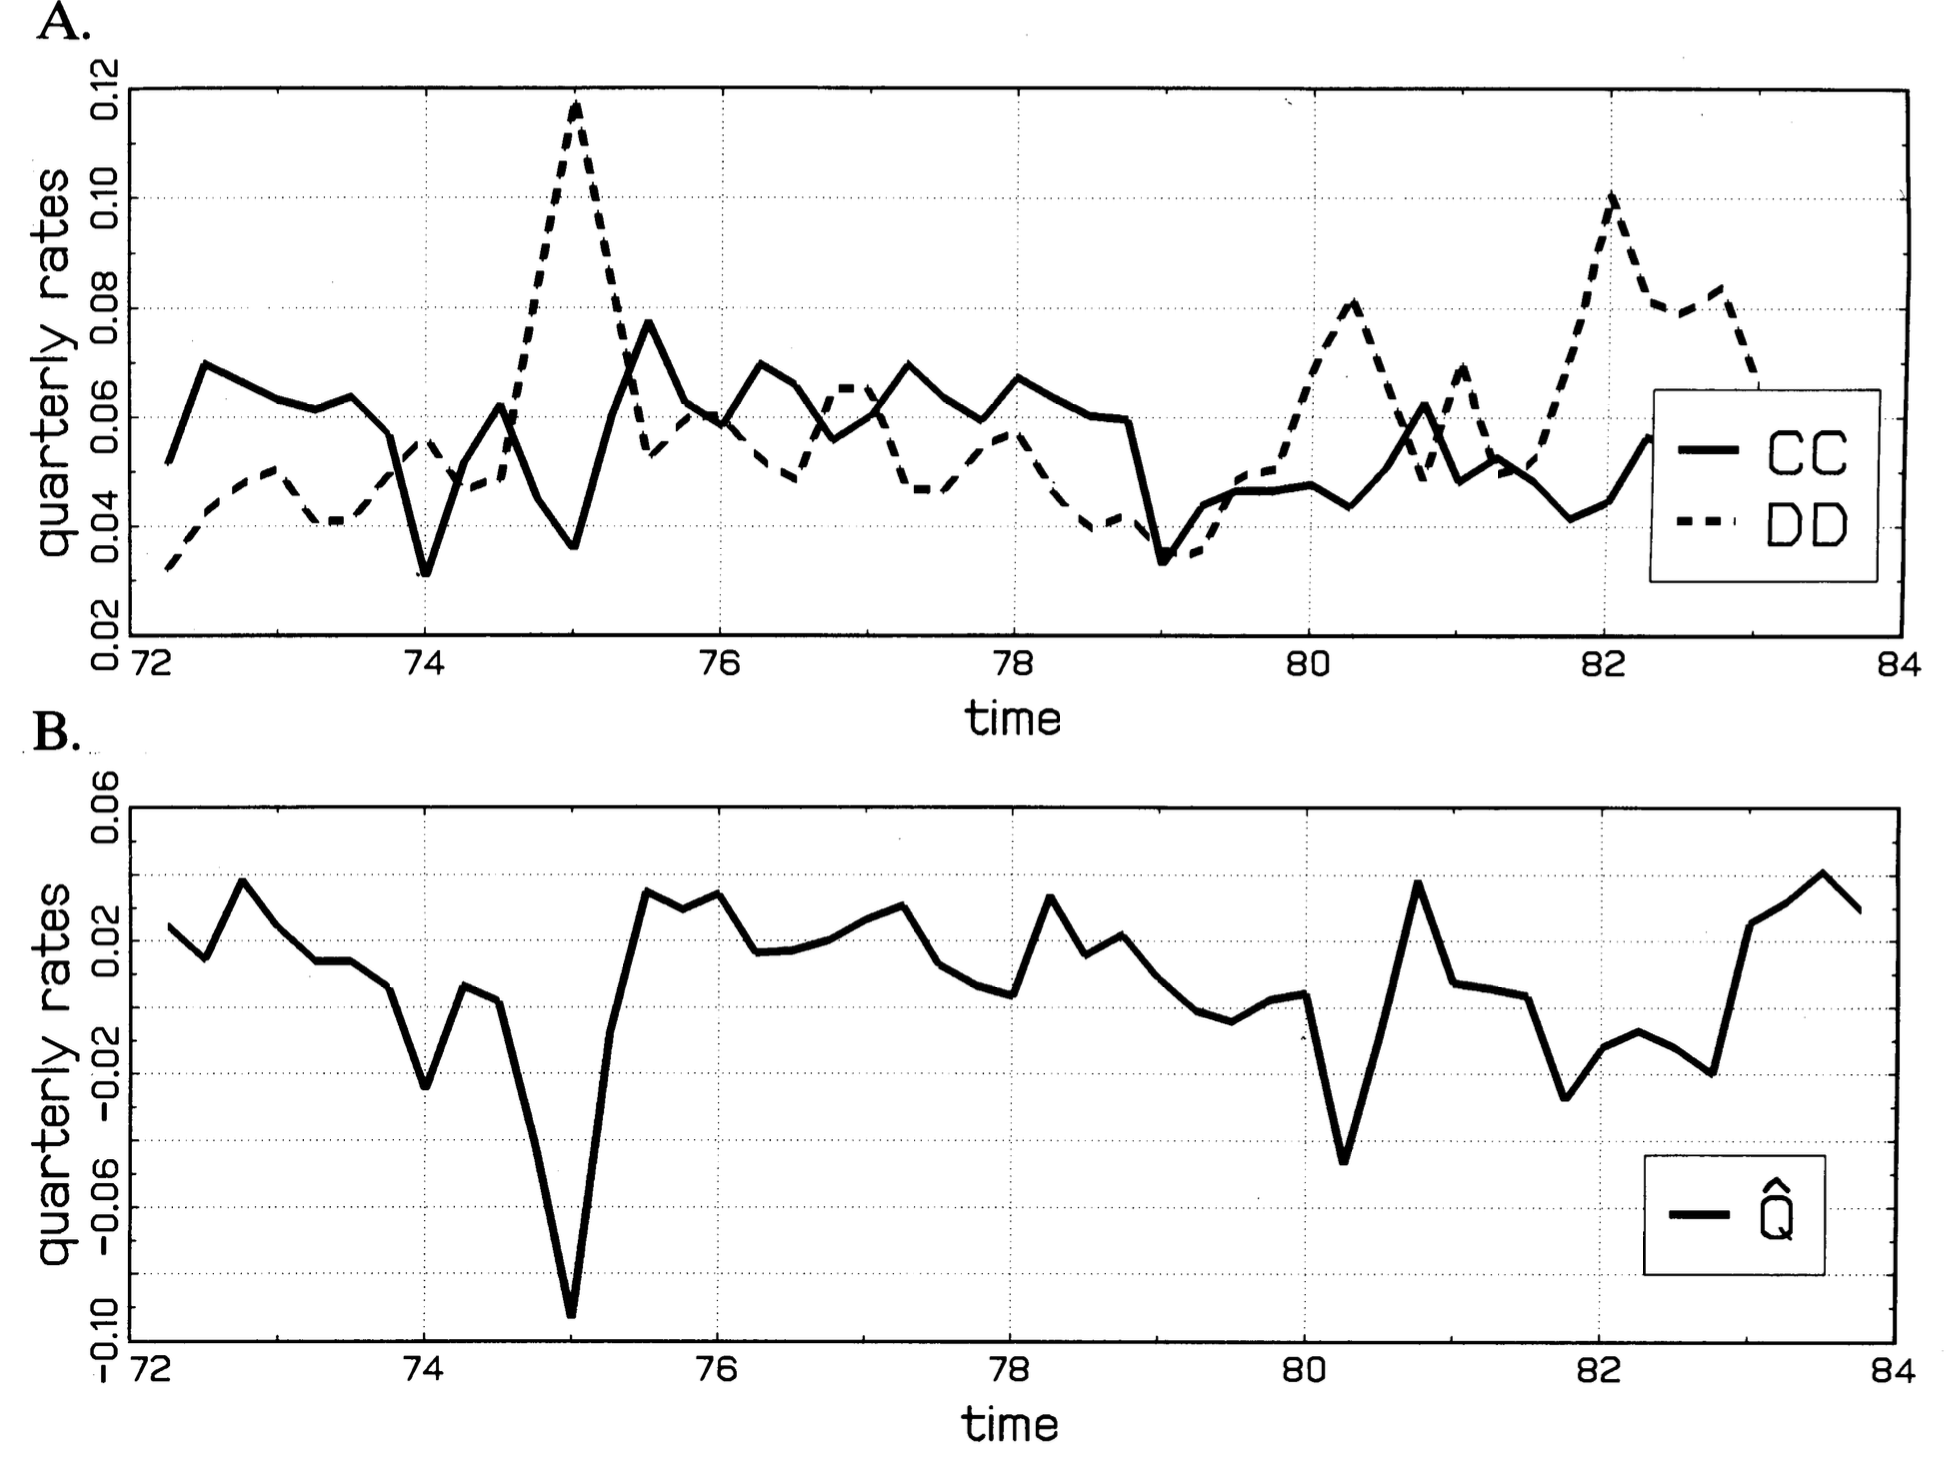
\includegraphics[scale = 0.4]{Plot2.2.png}
    \caption{Figure 1. Job creation and job destruction in U.S. Manufacturing B Index of the industrial production}
    \label{plot:2.2}
\end{figure}

To discern the characteristics of the series, the authors perform regression analysis on sectoral rates of job creation
and job destruction against leads and lags of the corresponding rates of growth. They find that job creation is less
responsive to demand fluctuations, while job destruction exhibits a more countercyclical behavior. 
\begin{figure}
    \centering
    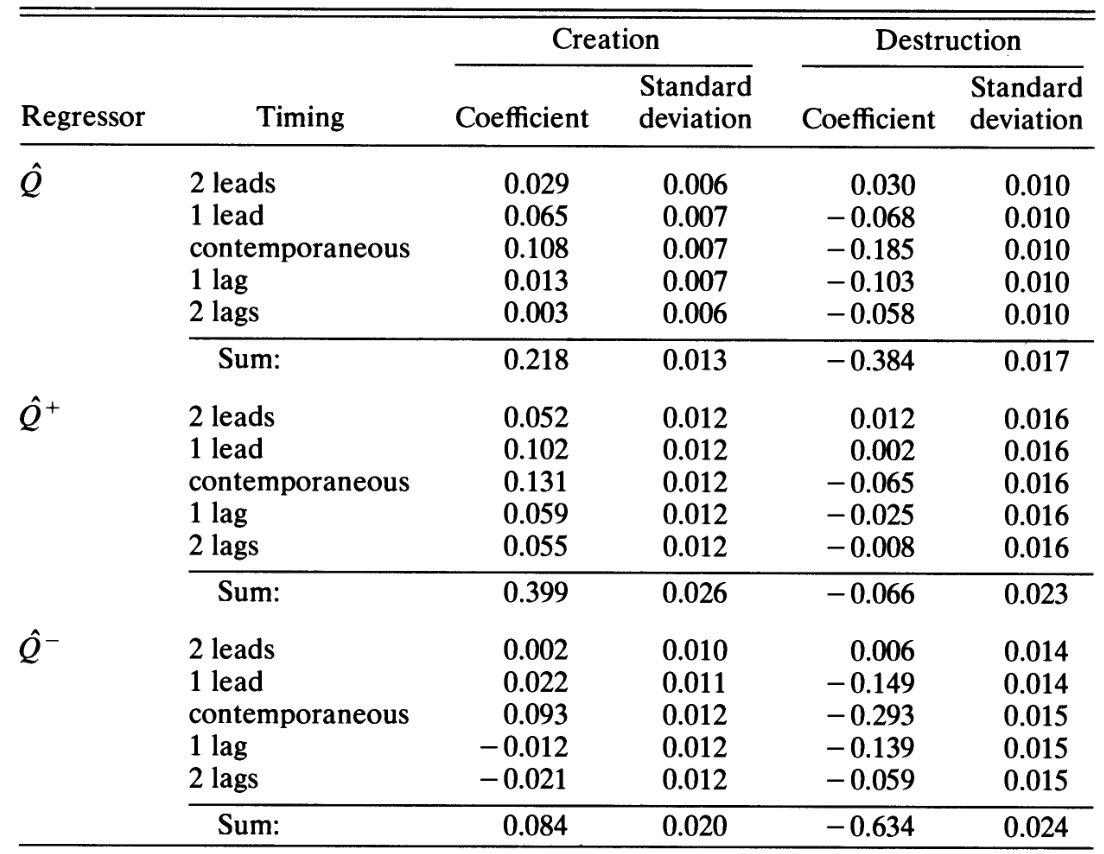
\includegraphics[scale = 0.4]{Plot2.3.png}
    \caption{Table 2.1. Job Creation and Job Destruction in U.S. Manufacturing Response to Output Growth}
    \label{Table 2.1.}
    \footnotesize \textit{Notes}: The table presents the reaction of job creation to the growth rate of the industrial
    production index. The latter is categorized into values above and below its mean (Q). The table encompasses
    quarterly observations for the two-digit SIC industries during the period 1972:2-1986:4. The coefficients are
    uniformly constrained to be equal across all sectors, with the exception of a constant (not shown).  
\end{figure}
The initial finding indicates that the rate of job destruction displays greater responsiveness to changes in sectoral
activity compared to the rate of job creation. Specifically, the sums of coefficients are -0.384 for job destruction and
0.218 for job creation showed in the table \ref{Table 2.1.}, the same results as in \cite{DAvHalt90,DavHalt92} and in
\cite{BlaDia90}.
The authors capitalize on a natural experiment rooted in the intrinsic asymmetric characteristics of business cycles.
Recessions, marked by brevity but intense contractions, provide the backdrop for the authors' model. This model
endeavors to emulate the creation rate while concurrently mitigating the impact of asymmetric cyclicality inherent in
business cycles. The empirical evidence supporting this model's behavior is encapsulated in Table \ref{Table 2.1.},
wherein two distinct scenarios are explored: output growth trajectories above \(Q^+\) and below \(Q^-\), relative to
their respective means. The table meticulously delineates how creation and destruction rates respond to these deviations
in output growth. 
\par
The salient observation emerges regarding creation rates, elucidating that they exhibit a more rapid and robust response
in instances of vigorous output growth, as opposed to scenarios where the output growth rate experiences a reduction. On
a contrasting note, the destruction margin, in line with the model's projections, manifests heightened sensitivity to a
decline in output. This responsiveness is particularly pronounced from one quarter before the onset of the shock to one
quarter after. Notably, during expansionary phases, the mean response of the destruction margin is -0.066, a notably
milder reaction compared to the recessionary case where the mean response stands at -0.634. 
\par
These empirical outcomes seamlessly align with the predictions of the model. Specifically, the creation rate exhibits
heightened responsiveness during expansionary phases, given their cyclical and symmetric nature. In contrast, the
asymmetric and non-cyclical nature of recessions triggers a more substantial decline in the production unit rate, in
line with the model's expectations. 
\par 
In oder to better understand the asymmetrical behavior the authors simulate an asymmetrical demand function:
\[\cdot{\overline{D}}(t)=0.05[\cos(t)+\sin(t)] - 0.016 \sin(2t)-0.003\cos(3t)\]
\[\overline{D}(t)=1\quad r = 0.065, \delta =0.15, \gamma=0.028, c_0=0.3, c_1=1.0\] 
The results are depicted in \ref{plot:2.4}
\begin{figure}
    \centering
    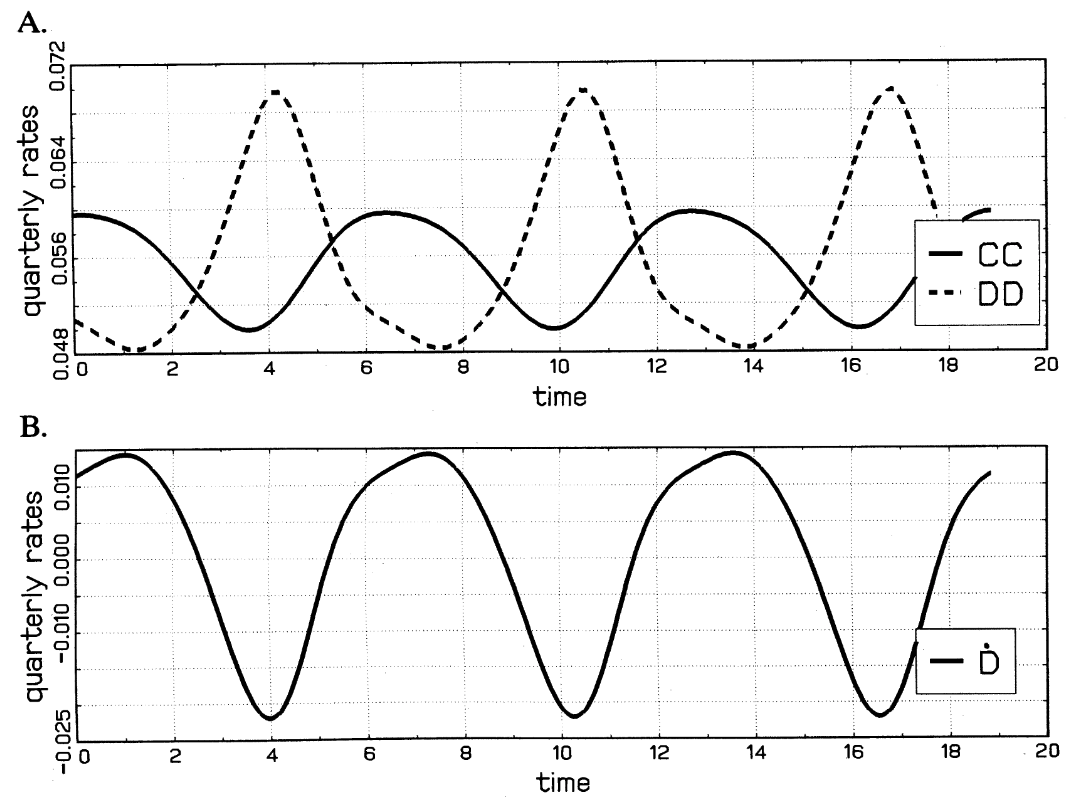
\includegraphics[scale = 0.4]{Plot2.4.png}
    \caption{A.  Creation and  Destruction B. Output Growth}
    \label{plot:2.4}
    \footnotesize \textit{Notes}: The figure depicts a simulation of asymmetrical supply growth.
\end{figure}

From the plot \ref{plot:2.4}, its evident that firms use prediction in demand to smooth job creation in order to avoid
big change, since they are too costly,by avaraging the demand over the lifetime of a production unit ove. On the other
hand, destruction depends only on current conditions, thus responding only to significant deviations from the demand
prediction . It can be better undestand thinking about a case in which creation rates respond only mildy to a sharp
deacrease in demand, the equilibrium price falls leading to additional distruction, since older units' profits go to 0.
Indeed, destruction not only preserves , but amplifies the assymetry of demand.\section{Frictionless economy}
\par
The authors culminate their study with a compelling calibration exercise using manufacturing series to exploit the
model. This entails dissecting the observed net change in employment into destruction and creation rates, as well as
applying the same approach to output production. The model is simulated for the duration of 1972:2-1983:4, with
parameters as follows: 

\begin{equation}
    \begin{aligned}
    &\text { Table 2.1 \label{Tab2.1} - Calibrated Parameters }\\
    &\begin{array}{lcc}
    \hline \hline \text { Variable } & \text { Symbol } & \text { Value } \\
    \hline \text { Interest rate } & r & 0.065 \\
    \text { Depreciation rate } & \delta & 0.150 \\
    \text { Rate of technical progress } & \gamma & 0.028 \\
    \text { Adjustment cost parameters } & c_0 & 0.403 \\
    & c_1 & 0.500 \\
    \hline
    \end{array}
    \end{aligned}
\end{equation}

The technical progress is selected to attribute all the growth in employment and manufacturing to technological
advancements, setting \(\lambda\) as 2.8. The authors employ Equation \ref{eq2.9}, linking the steady state to the
lifetime of jobs and job turnover (\(CC^*\)), determining \(\overline{a}^*+7.42\) years. Utilizing this information,
they ascertain the steady state entry cost to be 0.525, equivalent to half a year's operating costs for production
units. Subsequently, they employ ordinary least squares (OLS) to retrieve the value of \(c_1\), the marginal cost of
creating a new unit, which is found to be 0.5. This aligns with a small elasticity for the creation cost function,
signifying the vulnerability of the insulation mechanism to breakdown. 
\begin{figure}
    \centering
    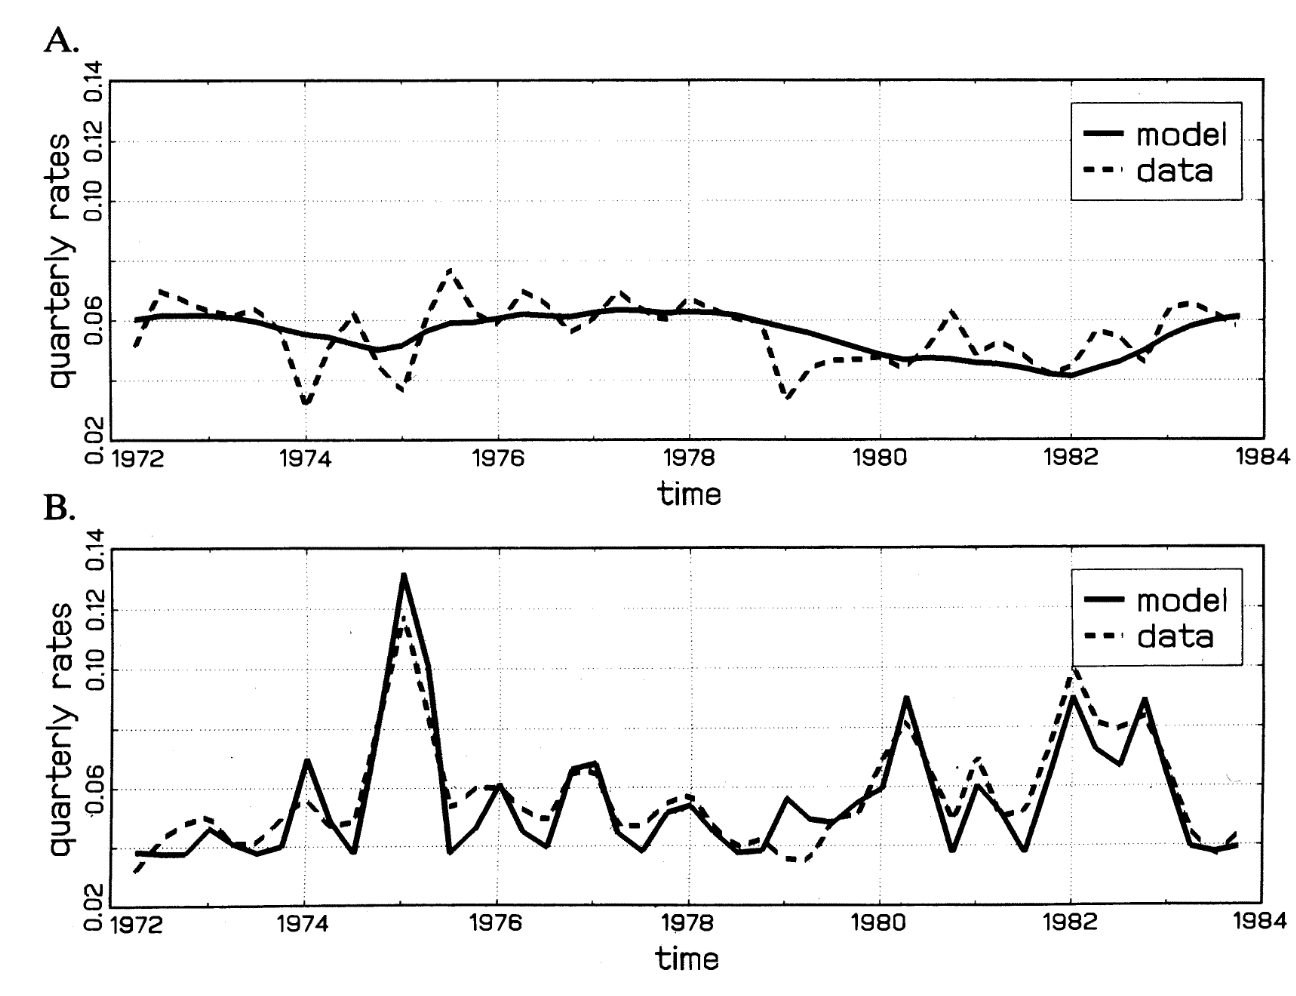
\includegraphics[scale = 0.6]{Plot2.5.png}
    \caption{Figure 1. A employment driven job creation \(c_0=0.403, c_1=0.5\) B Employment job destruction \(c_0=0.403, c_1=0.5\)} 
    \label{plot:2.5}
\end{figure}
The outcomes stemming from the simulations driven by employment and output are disclosed and contrasted with the data in
Figure \ref{plot:2.5}. Notably, the simulation of job creation displays a level of smoothness that diverges from the
observed 
data, with this discrepancy being attributed, in part, to the inherent absence of uncertainty in our model. Despite
this, the model effectively elucidates the relative volatility discernible in the patterns of job creation and
destruction. Moreover, it successfully captures the greater symmetry observed in the former, offering insights into the
nuanced dynamics at play in employment and output fluctuations. 
\par
The model provides intriguing insights as it elucidates certain empirical findings found in \cite{DAvHalt90,DavHalt92}.
Specifically, it delves into the dynamics of how the response of the creation margin contributes to an insulating effect
on the destruction margin. The model's salient features lie in its incorporation of heterogeneity across production
units and their turnover, rendering it a meaningful baseline for comprehending how the cleansing effect influences the
distribution of production units. 

However, it's essential to note that the model, in its current formulation, does not account for the potential impact of
financial frictions arising from asymmetric information between borrowers and lenders. Such frictions could conceivably
influence both the destruction and creation margins, introducing a layer of complexity not considered in the current
framework. 

An alternative perspective on recessions is captured by the concept of a "pit-stop," where a recession is characterized
as a period during which improvement investments in production are undertaken due to temporarily low opportunity costs,
as posited by \cite{DAvHalt90}. This viewpoint adds nuance to the understanding of recessions, emphasizing them as
periods conducive to strategic investments. 

One potential objection to the notion that recessions are times of cleansing is rooted in the implication of
countercyclical productivity. Notably, labor productivity is often observed to be procyclical. However, this apparent
inconsistency can be attributed to frictions, as suggested by \cite{GaHam92}. Their findings provide evidence supporting
the notion that the cleansing effect enhances productivity in the long term, offering a nuanced perspective on the
relationship between economic downturns and productivity dynamics. 
\par
A crucial observation in the aforementioned model is the authors' reliance on a constant marginal cost of creation. Yet,
recent literature has raised concerns about the reliability of this assumption, especially for larger firms. The
dynamics of the business environment in recent years suggest that significant firms tend to favor substantial
adjustments, particularly in terms of downsizing. 
\par
Interestingly, this deviation from the constant marginal adjustment cost for bigger firms can be interpreted as a
validation of the model's predictions. When firms opt not to fully insulate themselves from a decline in demand using
the creation margin, they tend to respond with intense layoffs. This alignment between the model's predictions and the
observed behavior of larger firms underlines the model's relevance and its capacity to capture real-world dynamics. 

\section{Solving}

Given that the evolution of the net worth is the following:
\[e_{t+1} = Z(\theta +\epsilon)k_t^\alpha + (1-\delta )k_t - (1+r)(c+k_t-e_t)\]
The value of the firm at time t is given by:
\[V_t(e_t) =\max_{k_t}  e_t + \beta V_{t+1}(e_{t+1})\]

Solving the Belman equation, the FOC are given by:
\[\frac{\vartheta V_t(e_t)}{\vartheta k_t } =\frac{\vartheta e_t}{\vartheta k_t } +
 \beta \frac{\vartheta V_{t+1}(e_{t+1})}{\vartheta k_t } \]
Strong assumption a change in \(k_t\) does not have an impact on \(e_t\) only on \(e_{t+1}\):
\[\frac{\vartheta e_t}{\vartheta k_t} = 0\]
Using the envelope theorem:
\[\frac{\vartheta
V_{t+1}(e_{t+1})}{\vartheta k_t } = \frac{\vartheta
V_{t+1}(e_{t+1})}{\vartheta e_{t+1} }\frac{\vartheta e_{t+1}}{\vartheta k_t}\]
\[\frac{\vartheta V_{t+1}(e_{t+1})}{\vartheta e_{t+1} } =1 + \beta(1+r)\]
\[\frac{\vartheta e_{t+1}}{\vartheta k_t} = Z(\theta +\epsilon)\alpha k_t^{\alpha-1}
-(\delta + r)\]
Thus:
\[\frac{\vartheta V_{t+1}(e_{t+1})}{\vartheta k_t } = 
[1+\beta(1+r)] [Z(\theta + \epsilon)\alpha k_t^{\alpha-1}-(\delta + r)] \]
So the FOC became:
\[\frac{\vartheta V_t(e_t)}{\vartheta k_t } = 0 + \beta [1+\beta(1+r)] [Z(\theta + \epsilon)\alpha
k_t^{\alpha-1}-(\delta + r)]  = 0 \]
The optimal level of capital at time t is:
\[\widehat{k} _t= {\frac{\beta(1+r) Z(\theta +\epsilon)\alpha}{\delta + r}}^{\frac{1}{1-\alpha}} \]
Plotting the graph in (assuming \(X=Z(\theta +\epsilon)\)) and \(y=\widehat{k} _t\)
\[ y={\frac{0.8 x}{0.03+0.1}}^{\frac{1}{1-0.8}}\]

\begin{figure}
    \centering
    \includegraphics[scale = 0.8]{K.png}
    \caption{\(X=Z(\theta +\epsilon)\) and \(y=\widehat{k} _t\) }
    \label{plot:k_static}
\end{figure}
Its interesting to see that if there is an increase in productivity the firm need more optimal capital K, while the most
low productivity firms need less capital to operate 


\subsection{Frictions}
Now I consider the participation constraint of the borrower given that she could observe \(\epsilon\) only paying \(\mu
k^\alpha\) so:
\[
 (1+r )(k+c+e)(1-\Phi(\overline{\epsilon}))+\int_{-\infty}^{\overline{\epsilon}}[Z(\theta+\overline{\epsilon})
k^\alpha+(1-\delta)k-\mu k^\alpha] \,d\Phi(\epsilon) \geq (1+r)(c+k+e)
 \]
\(r\) is the rate of interest that makes equal the expected value of borrowing to the opportunity cost of capital.
rewriting became 
\[
Z[\theta+G(\overline{\epsilon} )]k_t^\alpha+(1-\delta)k_t-uk_t^\alpha\Phi (\overline{\epsilon})=(1+r)(k_t+c-e_t)
\]
where
\[G(\overline{\epsilon} )= (1-\Phi(\varepsilon )\overline{\varepsilon }
+\int_{-\infty}^{\overline{\varepsilon}}\epsilon\,d \Phi(\epsilon) )\]
While the firm participation constraint is \(q_t \geq 0 \) so the end-of-period net worth must be greater than 0, thus
the problem of the firm becomes:
The value of the firm at time t is given by:
\[V_t(e_t) =\max_{k_t}  q_t - e_{t+1} + \beta V_{t+1}(e_{t+1})\]
\[s.t.\]
\[q_{t} = Z(\theta +\epsilon)k_t^\alpha + (1-\delta )k_t - (1+r)(c+k_t-e_t)\]
\[
Z[\theta+G(\overline{\epsilon} )]k_t^\alpha+(1-\delta)k_t-uk_t^\alpha\Phi (\overline{\epsilon})=(1+r)(k_t+c-e_t)
\]
so we can rewrite the second constraint in order to get \(r\):
\[r = \frac{Z[\theta+G(\overline{\epsilon} )]k_t^\alpha+(1-\delta)k_t-uk_t^\alpha\Phi (\overline{\epsilon})}{k_t+c-e_t}-1\]
FOC:
\[\frac{\vartheta
V_{t}(e_{t})}{\vartheta k_t } = \frac{\vartheta
q_{t}}{\vartheta k_t } - \frac{\vartheta
e_{t}}{\vartheta k_t } + \beta \frac{\vartheta
V_{t+1}(e_{t+1})}{\vartheta k_{t} } = 0\]
by envelope theorem:
\[\frac{\vartheta
V_{t+1}(e_{t+1})}{\vartheta k_{t} } = \frac{\vartheta
V_{t+1}(e_{t+1})}{\vartheta e_{t+1} }\frac{\vartheta e_{t+1}}{\vartheta k_t}\]
Strong HP: \[\frac{\vartheta e_{t+1}}{\vartheta k_t} = 0\]
Qui non so se ha senso continuare perchè non ho nessun meccanismo che mi trasformi il net worth al tempo t in net worth
al periodo t+1, almeno che non includa la definzione di dividendo come \(d_t= q_t-e_{t+1}\), allora in questo caso
dovrei risolvere il problema con un langrangiana dato che la firm dovrebbe scegliere sia \(k\) che \(e\) net worth.
\section{Redefining the problem}
\[V(k_{t}) = \max_{k_{t+1}, e_{t+1}} d_t + \beta V(k_{t+1})\]
\[s.t.\]
\[f(k_t) = Z k_t^\alpha\]
\[f(k_t) = d_t + (c+k_{t-1}-e_{t-1})(1+r) + k_{t} - (c + k_{t}- e_{t}) - k_{-1}(1-\delta)\]
\[(1+r)(c+k_t -e_t)p + (1-p)f(k_t) = (1+r_f)(c+k_t -e_t) \]
\[B_t = c+k_t-e_t; R= 1+r; R_f= 1 + r_f;  \]
\[R=\frac{R_f}{p}  -\frac{ 1-p }{ p }\frac{f(k_t)}{D_t}\]
In order to understand the mechanism behind this optimization problem, I firstly solve the three times problem working
backward.
The value function in \(t=2\) is 
\[ V_{t+2} =  \max d_{t+2}\]
Since there firm will not exists in t+2, there are no investiment \(B_{t+2}=0\), thus \(0=k_{t+2}+c-e_{t+2}\) as
consequence \(k_{t+2} = e_{t+2} - c\). Then we can rewrite the value function:
\[ V_{t+2} = \max Z(e_{t+2} - c)^\alpha - (c+k_{t+1}-e_{t+1})(1+r_{t+1}) - e_{t+2} + c + (c + e_{t+2} - c - e_{t+2}) +
k_{t+1}(1-\delta) \]
\[V_{t+2} = \max_{e_{t+2}} Z(e_{t+2} - c)^\alpha - B_{t+1}R_{l,t+1} - e_{t+2} + c + k_{t+1}(1-\delta) \]
FOC:
\[\frac{\partial V_{t+2}}{\partial e_{t+2}} = Z \alpha (e_{t+2} - c)^{\alpha-1} - 1 = 0\]
\[ (e_{t+2} - c)^{\alpha-1}= (Z \alpha)^{-1}\]
\[ e_{t+2} = (Z \alpha)^{\frac{1}{1-\alpha}}+c\]
Thus:
\[d_{t+2} = Z\left[(Z \alpha)^{\frac{\alpha}{1-\alpha}}\right]  - B_{t+1}R_{t+1} -  \left[(Z
\alpha)^{\frac{1}{1-\alpha}}\right] + k_{t+1}(1-\delta) \]
\[V_{t+2} = Z\left[(Z \alpha)^{\frac{\alpha}{1-\alpha}}\right]  - B_{t+1}R_{t+1} -  \left[(Z
\alpha)^{\frac{1}{1-\alpha}}\right] + k_{t+1}(1-\delta) \]
Writing the problem in t+1:
\[V_{t+1} = \max_{e_{t+1},k_{t+1}} d_{t+1} + \beta V_{t+2}\]
\[d_{t+1} = Zk^\alpha_{t+1} - B_t R_L - k_{t+1} + B_{t+1} + k_t(1-\delta)\]
FOCs:
\begin{equation}
    \left\{\begin{array}{@{}l@{}}
        \frac{\partial V_{t+1}}{\partial e_{t+1}} = \frac{\partial d_{t+1}}{\partial e_{t+1}} + \beta \frac{\partial
            V_{t+2}}{\partial e_{t+1}} = 0  \\
        \frac{\partial V_{t+1}}{\partial k_{t+1}} = \frac{\partial d_{t+1}}{\partial k_{t+1}} + \beta \frac{\partial
            V_{t+2}}{\partial K_{t+1}} = 0 \\
    \end{array} \right .\,
\end{equation}
solving \(\frac{\partial d_{t+1}}{\partial e_{t+1}}\):
\[\frac{\partial d_{t+1}}{\partial e_{t+1}} = Z \alpha k_{t+1} ^{\alpha-1}\frac{\partial k_{t+1}}{\partial e_{t+1}}
 - \frac{\partial k_{t+1}}{\partial e_{t+1}} + \frac{\partial B_{t+1}}{\partial e_{t+1}}\]
\[\frac{\partial B_{t+1}}{\partial e_{t+1}} = \frac{\partial k_{t+1}}{\partial e_{t+1}} - 1\]
\[\frac{\partial d_{t+1}}{\partial e_{t+1}} = Z \alpha k_{t+1} ^{\alpha-1}\frac{\partial k_{t+1}}{\partial e_{t+1}} -
\frac{\partial k_{t+1}}{\partial e_{t+1}} + \frac{\partial k_{t+1}}{\partial e_{t+1}} - 1\]

solving \(\frac{\partial V_{t+2}}{\partial e_{t+1}}\):
\[\frac{\partial V_{t+2}}{\partial e_{t+1}} = - \left[\frac{\partial B_{t+1}R_{t+1}}{\partial e_{t+1}} - \frac{\partial
k_{t+1}}{\partial e_{t+1}} \left( 1-\delta \right) \right]\] 
\[\frac{\partial B_{t+1}R_{t+1}}{\partial e_{t+1}} = \frac{\partial B_{t+1}}{\partial e_{t+1}}R_{t+1} +
B_{t+1}\frac{\partial R_{t+1}}{\partial e_{t+1}} \]
\[\frac{\partial B_{t+1}}{\partial e_{t+1}} = \frac{\partial k_{t+1}}{\partial e_{t+1}}-1\]
\[\frac{\partial R_{t+1}}{\partial e_{t+1}} = - \frac{1-p}{p}\left\{\left[Z\alpha k^{\alpha-1}_{t+1}\frac{\partial
k_{t+1}}{\partial e_{t+1}} -\delta \frac{\partial k_{t+1}}{\partial e_{t+1}}\right] B_{t+1} - \left(\frac{\partial
k_{t+1}}{\partial e_{t+1}} - 1\right) \left[Zk_{t+1}^{\alpha} - \delta k_{t+1}\right]\right\}B_{t+1}^{-2}\]
\[\frac{\partial B_{t+1}R_{t+1}}{\partial e_{t+1}} = \left[\frac{\partial k_{t+1}}{\partial e_{t+1}}-1 \right] R_{t+1}
- \frac{1-p}{p}\left\{\left[Z\alpha k^{\alpha-1}_{t+1}\frac{\partial
k_{t+1}}{\partial e_{t+1}} -\delta \frac{\partial k_{t+1}}{\partial e_{t+1}}\right] B_{t+1} - \left(\frac{\partial
k_{t+1}}{\partial e_{t+1}} - 1\right) \left[Zk_{t+1}^{\alpha} - \delta k_{t+1}\right]\right\}B_{t+1}^{-1}\]
\[\frac{\partial B_{t+1}R_{t+1}}{\partial e_{t+1}} = \left(\frac{\partial k_{t+1}}{\partial e_{t+1}} -1
\right)\left[\left(zk^\alpha_{t+1} -\delta k_{t+1}\right)\frac{1-p}{p}B_{t+1}^{-1}+R_{t+1}\right] -
\frac{1-p}{p}\frac{\partial k_{t+1}}{\partial e_{t+1}} \left(Z\alpha k^{\alpha-1}_{t+1} - \delta\right)\]
\[\frac{\partial B_{t+1}R_{t+1}}{\partial e_{t+1}} = \left(\frac{\partial k_{t+1}}{\partial e_{t+1}} -1
\right)R_f-
\frac{1-p}{p}\frac{\partial k_{t+1}}{\partial e_{t+1}} \left(Z\alpha k^{\alpha-1}_{t+1} - \delta\right)\]
\[\frac{\partial V_{t+2}}{\partial e_{t+1}} = - \left[\left(\frac{\partial k_{t+1}}{\partial e_{t+1}} -1
\right)R_f-
\frac{1-p}{p}\frac{\partial k_{t+1}}{\partial e_{t+1}} \left(Z\alpha k^{\alpha-1}_{t+1} - \delta\right) - \frac{\partial
k_{t+1}}{\partial e_{t+1}} \left( 1-\delta \right)\right]\]
Substituting into the first FOC, we get:
\[\frac{\partial V_{t+1}}{\partial e_{t+1}} = Z \alpha k_{t+1} ^{\alpha-1}\frac{\partial k_{t+1}}{\partial e_{t+1}} -
\frac{\partial k_{t+1}}{\partial e_{t+1}} + \frac{\partial k_{t+1}}{\partial e_{t+1}} - 1 - \beta 
\left[\left(\frac{\partial k_{t+1}}{\partial e_{t+1}} -1 
\right)R_f-
\frac{1-p}{p}\frac{\partial k_{t+1}}{\partial e_{t+1}} \left(Z\alpha k^{\alpha-1}_{t+1} - \delta\right) - \frac{\partial
k_{t+1}}{\partial e_{t+1}} \left( 1-\delta \right)\right] = 0\]
second FOC: \\
solving \(\frac{\partial d_{t+1}}{\partial k_{t+1}}\):
\[\frac{\partial d_{t+1}}{\partial k_{t+1}} = Z \alpha k_{t+1} ^{\alpha-1} - 1 + \frac{\partial B_{t+1}}{\partial
k_{t+1}} \]
\[\frac{\partial B_{t+1}}{\partial
k_{t+1}} = 1 - \frac{\partial e_{t+1}}{\partial k_{t+1}} \]
\[\frac{\partial d_{t+1}}{\partial k_{t+1}} = Z \alpha k_{t+1} ^{\alpha-1} - \frac{\partial e_{t+1}}{\partial
k_{t+1}}\]
solving \(\frac{\partial V_{t+2}}{\partial k_{t+1}}\):
\[\frac{\partial V_{t+2}}{\partial k_{t+1}} = -\left[\frac{\partial B_{t+1}R_{t+1}}{\partial k_{t+1}} -(1-\delta)\right] \]
\[\frac{\partial B_{t+1}R_{t+1}}{\partial k_{t+1}} = \frac{\partial B_{t+1}}{\partial k_{t+1}}R_{t+1} +
B_{t+1}\frac{\partial R_{t+1}}{\partial k_{t+1}}\]
\[\frac{\partial B_{t+1}}{\partial k_{t+1}} = 1-\frac{\partial e_{t+1}}{\partial k_{t+1}} \]
\[\frac{\partial R_{t+1}}{\partial k_{t+1}} =  - \frac{1-p}{p}\left[\left(Z\alpha k^{\alpha-1}_{t+1}-\delta\right)B_{t+1} -
\left(1-\frac{\partial e_{t+1}}{\partial k_{t+1}}\right)\left(Zk_{t+1}^{\alpha} - \delta k_{t+1}
\right)\right]B_{t+1}^{-2} 
\]
\[\frac{\partial B_{t+1}R_{t+1}}{\partial k_{t+1}} = \left(1-\frac{\partial e_{t+1}}{\partial k_{t+1}}\right) R_{t+1} +
\left\{\frac{1-p}{p}\left[(Z \alpha k^{\alpha-1}_{t+1}-\delta)B_{t+1} -
\left(1-\frac{\partial e_{t+1}}{\partial k_{t+1}}\right)\left(Zk_{t+1}^{\alpha} - \delta k_{t+1}
\right)\right]B_{t+1}^{-1} \right\}\]
\[\frac{\partial B_{t+1}R_{t+1}}{\partial k_{t+1}} =\left(1-\frac{\partial e_{t+}}{\partial k_{t+1}}\right)
\left[R_{t+1} + \frac{1-p}{p}\left(Z k_{t+1}^{\alpha} - \delta k_{t+1}\right)B_{t+1}^{-1}\right]-
\frac{1-p}{p}\left(Z\alpha k^{\alpha-1}_{t+1}-\delta\right) \]
\[\frac{\partial B_{t+1}R_{t+1}}{\partial k_{t+1}} =\left(1-\frac{\partial e_{t+1}}{\partial k_{t+1}}\right)
R_f - \frac{1-p}{p}\left(Z\alpha k^{\alpha-1}_{t+1}-\delta\right) \]
\[\frac{\partial V_{t+2}}{\partial k_{t+1}} = -\left[\left(1-\frac{\partial e_{t+1}}{\partial k_{t+1}}\right)
R_f - \frac{1-p}{p}\left(Z\alpha k^{\alpha-1}_{t+1}-\delta\right)- \left(1-\delta\right)\right] \]
Substituting into the FOC:
\[\frac{\partial V_{t+1}}{\partial k_{t+1}} =Z \alpha k_{t+1} ^{\alpha-1} - \frac{\partial e_{t+1}}{\partial
k_{t+1}} - \beta \left[\left(1-\frac{\partial e_{t+1}}{\partial k_{t+1}}\right)
R_f - \frac{1-p}{p}\left(Z\alpha k^{\alpha-1}_{t+1}-\delta\right)- \left(1-\delta\right)\right]=0\]
thus the FOCs are:
\[\frac{\partial V_{t+1}}{\partial e_{t+1}} = Z \alpha k_{t+1} ^{\alpha-1}\frac{\partial k_{t+1}}{\partial e_{t+1}}  - 1 - \beta 
\left[\left(\frac{\partial k_{t+1}}{\partial e_{t+1}} -1 
\right)R_f-
\frac{1-p}{p}\frac{\partial k_{t+1}}{\partial e_{t+1}} \left(Z\alpha k^{\alpha-1}_{t+1} - \delta\right) - \frac{\partial
k_{t+1}}{\partial e_{t+1}} \left( 1-\delta \right)\right] = 0\]
\[\frac{\partial V_{t+1}}{\partial k_{t+1}} =Z \alpha k_{t+1} ^{\alpha-1} - \frac{\partial e_{t+1}}{\partial
k_{t+1}} - \beta \left[\left(1-\frac{\partial e_{t+1}}{\partial k_{t+1}}\right)
R_f - \frac{1-p}{p}\left(Z\alpha k^{\alpha-1}_{t+1}-\delta\right)- \left(1-\delta\right)\right]=0\]
rearranging \(\frac{\partial V_{t+1}}{\partial k_{t+1}} \) to isolate \(k_{t+1}\):
\[k^{\alpha-1}_{t+1}=\left[\frac{\partial e_{t+1}}{\partial k_{t+1}}\left(1-\beta R_f\right) + \beta
\left(r_f+\frac{\delta}{p}\right)\right]\left\{Z\alpha\left[\left(1-\beta\right)-\frac{\beta}{p}\right]\right\}^{-1}\] 
rearranging \(\frac{\partial V_{t+1}}{\partial e_{t+1}} \) to isolate \(k_{t+1}\):
\[k^{\alpha-1}_{t+1}=\left[\frac{\partial k_{t+1}}{\partial e_{t+1}}\left(1-\beta R_f\right) + \beta
\left(r_f+\delta\right) + \delta \frac{1-p}{p}\right]\frac{p}{Z\alpha}\]
Equating the two equations:
\[\left[\frac{\partial e_{t+1}}{\partial k_{t+1}}\left(1-\beta R_f\right) + \beta
\left(r_f+\frac{\delta}{p}\right)\right]\left\{Z\alpha\left[\left(1-\beta\right)-\frac{\beta}{p}\right]\right\}^{-1} =
\left[\frac{\partial k_{t+1}}{\partial e_{t+1}}\left(1-\beta R_f\right) + \beta 
\left(r_f+\delta\right) + \delta \frac{1-p}{p}\right]\frac{p}{Z\alpha}\]
From this equation, you can isolate \(\frac{\partial e_{t+1}}{\partial k_{t+1}}\) to solve for it explicitly.
\[\frac{\partial e_{t+1}}{\partial k_{t+1}} = -\left[\frac{\partial k_{t+1}}{\partial e_{t+1}}\left(1-\beta R_f\right) + \beta
\left(r_f+\delta\right) + \delta
\frac{1-p}{p}\right]\frac{p}{Z\alpha}\left\{Z\alpha\left[\left(1-\beta\right)-\frac{\beta}{p}\right]\right\}\left(1-\beta
R_f\right)^{-1} - \beta \left(r_f+\frac{\delta}{p}\right)\left(1-\beta R_f\right)^{-1}\] 
\[\frac{\partial e_{t+1}}{\partial k_{t+1}} =- \left[\frac{\partial k_{t+1}}{\partial e_{t+1}}\left(1-\beta R_f\right)
+\delta\frac{1-p}{p}\right]\frac{\beta p +\beta -p}{1-\beta R_f} - \beta \left(r_f+\frac{\delta}{p}\right)\left(1-\beta
R_f\right)^{-1} \]
Since \(\frac{\partial e_{t+1}}{\partial k_{t+1}}\) is the reciprocal of \(\frac{\partial k_{t+1}}{\partial e_{t+1}}\),
we can compute the optimal path of the networth as a function of the capital.
Defining \(y =\frac{\partial e_{t+1}}{\partial k_{t+1}}\) and ths \(\frac{y^{-1}=\partial e_{t+1}}{\partial k_{t+1}}\):
\[y= - \left[\frac{1}{y}\left(1-\beta R_f\right)
+\delta\frac{1-p}{p}\right]\frac{\beta p +\beta -p}{1-\beta R_f} - \beta \left(r_f+\frac{\delta}{p}\right)\left(1-\beta
R_f\right)^{-1} \]
To solve the given equation \[y= - \left[\frac{1}{y}\left(1-\beta R_f\right)
+\delta\frac{1-p}{p}\right]\frac{\beta p +\beta -p}{1-\beta R_f} - \beta \left(r_f+\frac{\delta}{p}\right)\left(1-\beta
R_f\right)^{-1} \]


Use Python and the sympy library to solve the equation:
\begin{lstlisting}[language=Python]
from sympy import symbols, Eq, solve

# Define the symbols
y, beta, R_f, delta, p, r_f = symbols('y beta R_f delta p r_f')

# Define the equation
equation = Eq(y, - ((1/y) * (1 - beta * R_f) + delta * (1 - p) / p) * (beta * p + beta - p) / (1 - beta * R_f) - beta * (r_f + delta / p) / (1 - beta * R_f))

# Solve for y
solution = solve(equation, y)
\end{lstlisting}


The equation for \(y\) is given by:

\[y = \frac{\beta \delta \pm  \sqrt{\Delta}}{2 p (\beta  R_f - 1)}\]


In the solutions provided, \( \Delta \) represents the discriminant of the quadratic equation that was formed during the
solution process. It is the expression under the square root in the solutions. The discriminant \( \Delta \) in this
case is a complex expression involving the variables \( R_f \), \( \beta \), \( p \), \( \delta \), and \( r_f \).
Specifically, \( \Delta \) is given by: 

\begin{align}
    &\Delta = (-\beta \delta - \beta p^2 \delta\left(\frac{1}{p} - 1\right) + p^2 \delta\left(\frac{1}{p} - 1\right) \\
    &- \beta p \delta\left(\frac{1}{p} - 1\right) - \beta p r_f)^2 \\
    &- 4 (\beta p R_f - p) (\beta^2 p^2 R_f - \beta p^2 R_f + \beta^2 p R_f \\
    &- \beta p^2 + p^2 - \beta p)
\end{align}

The discriminant \( \Delta \) is given by:
\begin{equation}
    \Delta = \text{[complex expression involving \( R_f \), \( \beta \), \( p \), \( \delta \), and \( r_f \)]}
\end{equation}


The sign of the solutions depends on:
\begin{itemize}
    \item The values of \( \beta \), \( \delta \), \( p \), \( R_f \), and \( r_f \).
    \item The value and sign of \( \Delta \).
\end{itemize}
Since \( \Delta \) involves these parameters in a complex manner, the sign of the solutions can be:
\begin{itemize}
    \item Real and positive, real and negative, or complex (depending on the sign and magnitude of \( \Delta \) and other parameters).
    \item Determined specifically only when actual values for the parameters are provided.
\end{itemize}
Since now we have a partial derivative as a function of parametrs we can retrive the relation between equity and
capital.
Rewriting the solutions as:
\[y =\frac{\partial e_{t+1}}{\partial k_{t+1}}= \frac{N}{D}\]
Given the partial derivative:
\begin{equation}
    \frac{\partial e_{t+1}}{\partial k_{t+1}} = \frac{N}{D}
\end{equation}
where \(N\) and \(D\) are constants with respect to \(k\), we want to integrate this with respect to \(k\).

Since \(N\) and \(D\) do not depend on \(k\), the integral is straightforward:
\begin{equation}
    \int \frac{N}{D} \, dk
\end{equation}

Integrating a constant with respect to \(k\) yields:
\begin{equation}
    \int \frac{N}{D} \, dk = \frac{N}{D} \cdot k + C
\end{equation}
where \(C\) is the constant of integration.

Thus, the set of possible solutions is:
\begin{equation}
    e_{t+1} = \frac{N}{D} \cdot k_{t+1} + C
\end{equation}
where \(C\) is determined based on boundary conditions or initial values.
Given the relationship:
\begin{equation}
    k^{\alpha-1}_{t+1} = \left[\frac{\partial e_{t+1}}{\partial k_{t+1}}\left(1-\beta R_f\right) + \beta \left(r_f+\frac{\delta}{p}\right)\right]\left\{Z\alpha\left[\left(1-\beta\right)-\frac{\beta}{p}\right]\right\}^{-1}
\end{equation}
we can retrieve \(k_{t+1}\).

Substituting \(\frac{\partial e_{t+1}}{\partial k_{t+1}} = \frac{N}{D}\) into the equation, we get:
\begin{equation}
    k^{\alpha-1}_{t+1} = \left[\frac{N}{D}\left(1-\beta R_f\right) + \beta \left(r_f+\frac{\delta}{p}\right)\right]\left\{Z\alpha\left[\left(1-\beta\right)-\frac{\beta}{p}\right]\right\}^{-1}
\end{equation}
Sine now we have the optimal k we can retrieve the optimal path of networth:
\[e_{t+1} = \frac{N}{D} \cdot \left[\frac{N}{D}\left(1-\beta R_f\right) + \beta
\left(r_f+\frac{\delta}{p}\right)\right]\left\{Z\alpha\left[\left(1-\beta\right)-\frac{\beta}{p}\right]\right\}^{-1} +
C\]
Thus the debt at time t+1 is:
\begin{align}
    B_{t+1} = & \left[\frac{N}{D}\left(1-\beta R_f\right) + \beta\left(r_f+\frac{\delta}{p}\right)\right]\left\{Z\alpha\left[\left(1-\beta\right)-\frac{\beta}{p}\right]\right\}^{-1} + c \nonumber \\
    & - \left\{\frac{N}{D} \cdot \left[\frac{N}{D}\left(1-\beta R_f\right) + \beta\left(r_f+\frac{\delta}{p}\right)\right]\left\{Z\alpha\left[\left(1-\beta\right)-\frac{\beta}{p}\right]\right\}^{-1} + C\right\}
\end{align}




% Fino a qui non ho molti dubbi, mentre il seguente passaggio presenta molti dubbi e secondo me è responsabile del segno
% negativo del capitale. Tuttavia non mi è venuto in mente altro modo per procedere.
% Knowing that \(B = k + c - e \rightarrow e= B -k -c\) thus \(\frac{\partial e_{t+1}}{\partial k_{t+1}} = -1\):
% \[  -\beta \left(r_f+\frac{\delta}{p}\right)\left(1-\beta R_f\right)^{-1}\frac{1-\beta R_f}{\beta p +\beta -p}= \left[\frac{\partial k_{t+1}}{\partial e_{t+1}}\left(1-\beta R_f\right)
% +\delta\frac{1-p}{p}\right]\]


% We can rearrange it to isolate \(\frac{\partial k_{t+1}}{\partial e_{t+1}}\):

% \[ -\beta \left(r_f+\frac{\delta}{p}\right)\left(\beta p +\beta -p\right) - \delta\frac{1-p}{p} = \frac{\partial k_{t+1}}{\partial e_{t+1}}\left(1-\beta
% R_f\right)\] 

% Now, solve for \(\frac{\partial k_{t+1}}{\partial e_{t+1}}\) by dividing both sides by \((1-\beta R_f)\):

% \[\frac{\partial k_{t+1}}{\partial e_{t+1}} = \left\{-\beta \left(r_f+\frac{\delta}{p}\right)\left(\beta p +\beta
% -p\right) - \delta\frac{1-p}{p} 
% \right \} \left(1-\beta R_f\right)^{-1}\]

% This equation provides the value of \(\frac{\partial k_{t+1}}{\partial e_{t+1}}\) in terms of the given constants
% (\(\beta, R_f, p, \delta\)) and the relationship between \(e_{t+1}\) and \(k_{t+1}\). 
% \[k^{\alpha-1}_{t+1}=\left[\left\{-\beta \left(r_f+\frac{\delta}{p}\right)\left(\beta p +\beta
% -p\right) - \delta\frac{1-p}{p} 
% \right \} + \beta
% \left(r_f+\delta\right) + \delta \frac{1-p}{p}\right]\frac{p}{Z\alpha}\]
% \[k^{\alpha-1}_{t+1}= \left[\left\{-\beta \left(r_f+\frac{\delta}{p}\right)\left(\beta p +\beta
% -p\right) 
% \right \} + \beta
% \left(r_f+\delta\right) \right]\frac{p}{Z\alpha}\]

\medskip


\bibliography{reference}

\end{document}